\documentclass{uflamon}          % classe base para a monografia

%==============================================================================
\usepackage{rotating}

% Utilizacao de pacotes
\usepackage[T1]{fontenc}         % usa fontes postscript com acentos
\usepackage[brazil]{babel}       % hifenização e títulos em português do Brasil
\usepackage[utf8]{inputenc}     % permite edição direta com acentos
\usepackage{amsmath}             % pacote da AMS para Matemática Avançada
\usepackage{amssymb}             % símbolos extras da AMS
\usepackage{latexsym}            % símbolos extras do LaTeX
\usepackage{graphicx}            % para inserção de gráficos
\usepackage{listings}            % para inserção de código
\usepackage{fancyvrb}            % para inserção de saídas de comandos
%\usepackage{enumerate}           % para personalizar lista enumeradas 
											%(incluso na classe)
\usepackage{longtable}           % para tabelas muito grandes NOVO!!!!


\usepackage{epstopdf}



\usepackage{colortbl} % cores em tabelas
\newcolumntype{Z}{|>{\columncolor[gray]{0.9}}l|} %cor cinza em células
%\usepackage{array} % já incluso na classe
\newcolumntype{L}[1]{>{\raggedright\let\newline\\\arraybackslash\hspace{0pt}}m{#1}}
\newcolumntype{C}[1]{>{\centering\let\newline\\\arraybackslash\hspace{0pt}}m{#1}}
\newcolumntype{R}[1]{>{\raggedleft\let\newline\\\arraybackslash\hspace{0pt}}m{#1}}
\usepackage{multirow} % para juntar duas linhas em uma só

\usepackage{multicol} % para uso de várias colunas

% cores para os links cruzados
\usepackage{color}
\definecolor{rltred}{rgb}{0.2,0,0}
\definecolor{rltgreen}{rgb}{0,0.2,0}
\definecolor{rltblue}{rgb}{0,0,0.2}

\usepackage[colorlinks=true,
            urlcolor=rltblue,       % \href{...}{...} external (URL)
            filecolor=rltgreen,     % \href{...} local file
            linkcolor=rltred,       % \ref{...} and \pageref{...}
            citecolor=rltgreen,
            pdftitle={Sistema de Identificação de Condutores Baseado em Técnicas de Inteligência Computacional},
          pdfauthor={Andrey Gustavo de Souza},
          pdfsubject={},
          pdfkeywords={}%
]{hyperref} % para referência cruzadas
%\usepackage{hyperref}            % para referência cruzadas
\usepackage{subfigure}           % figuras dentro de figuras
\usepackage{caption}            % remodelando o formato dos títulos de 
                                 % tabelas e figuras

% configuração padrão do listings   
\lstset{
   language=Java,
   extendedchars=true,
   tabsize=3,
   basicstyle=\footnotesize\ttfamily,
   stringstyle=\em,
   showstringspaces=false 
}

% para referências de acordo com a ABNT
% precisa instalar o abntex2 antes!!!
% http://abntex.codigolivre.org.br/
% comente se pretende usar outro padrão

%abnt-emphasize=bf coloca o título das bibliografias em negrito
%abnt-thesis-year=both
\usepackage[alf,abnt-etal-cite=3,abnt-etal-list=3,abnt-url-package=url,abnt-emphasize=bf]{abntex2cite}

% evite usar o hyperref com abntex, pode dar caca em urls... no linha anterior, informo
% para incluir urls usando o pacote url e não o hyperref
%
% caso queira o hyperref com abntex, comente a linha anterior e descomente a seguinte
%\usepackage[alf,abnt-etal-cite=3,abnt-etal-list=0,abnt-etal-text=emph]{abntex2cite}
%
% caso vc ainda use a versão anterior da abntex, comente a linha incluindo o abntex2cite
% e descomente a próxima linha 
%\usepackage[alf,abnt-etal-cite=3,abnt-etal-list=0,abnt-etal-text=emph]{abntcite}


% redefinindo formatação de títulos de tabelas e figuras


%==============================================================================
% para os fãs do Word, descomente as linhas abaixo
%\sloppy %mais espaço entre as linhas
%\usepackage{identfirst} %identando-se a primeira linha de cada seção
%\noindentfirst % Tire o comentário para manter o padrão do LaTeX.

%==============================================================================
% definido comandos na monografia - não é necessário na sua monografia 
% apenas para exemplificar a definição de novos comandos
\newcommand{\defs}[1]{\textsl{#1}}


% Especificando hifenizações que por ventura LaTeX não saiba fazer
% Por padrão 99,9% dos termos em português devem ser hifenizados corretamente.
\hyphenation{hardware software Li-nux am-bien-te diag-nos-ti-car coor-de-na-ção 
FAE-PE Recovery TelEduc Williams UFLA}

%==============================================================================
% Dados da monografia, capa: autor, titulo, banca, etc... - SUBSTITUA DE ACORDO
%==============================================================================
\author{Andrey Gustavo de Souza}
\title{Sistema de Identificação de Condutores Baseado em Técnicas de Inteligência Computacional}

\date{2017}
\tipo{Projeto de pesquisa apresentado à Universidade Federal de Lavras, como parte das exigências do Programa de Pós-Graduação em Engenharia de Sistemas e Automação para a obtenção do título de Mestre.}
% use \orientador ou \orientadora quando for o caso
\orientador{Prof. Dr. Wilian Soares Lacerda}
%\orientadora{}
% use \coorientador ou \coorientadora quando for o caso
%\coorientador{Prof. Dr. Danilo Alves de Lima} % comente se não tiver coorientador
%%\coorientador{}
\local{Lavras -- MG}


%\bancaum{Prof. MSc. Antônio Banca Um}{UFM}
%\bancadois{Prof. DSc. João Banca Dois}{FCO} % comente se sua banca tiver só um professor
%\bancatres{Profa. Esp. Eliza Banca Três}{BELMIS}
%\bancaquatro{Prof. Esp. Carlos Banca Quatro}{IBGPLUS}
%\defesa{30 de Fevereiro de 2016}


%==============================================================================
%%##################################################
%% Dados para Ficha catalográfica, gerada pelo sistema da Biblioteca da UFLA
%% http://www.biblioteca.ufla.br/FichaCatalografica/
%% dados para ficha catalográfica
%% Elaboração da Ficha Catalográfica
%\preparofichacat{Ficha catalográfica elaborada pela Coordenadoria de Processos Técnicos \\ da Biblioteca Universitária da UFLA}
%% primeiro autor - como na primeira linha da ficha catalográfica
%\fcautor{Uchôa, Joaquim Quinteiro}
%% autores, separados por vírgula - na ficha catalográfica, no formato que
%% vem após o título e a barra ("/")
%\fcautores{Joaquim Quinteiro Uchôa}
%% caso trabalho seja ilustrado (figuras, gráficos, tabelas, etc.), 
%% então informar por meio do comando a seguir
%% caso não seja ilustrado, basta comentá-lo
%\fcilustrado{il.}
%% dados da edição para a ficha 
%\fcedicao{2$^a$ ed. rev., atual. e ampl.}
%% tipo do trabalho (tese, dissertação, etc.), de acordo com sistema
%% de geração de ficha catalográfica
%\fctipo{Tese(doutorado)}
%% ano da defesa, só precisa informar se for diferente do ano da publicação
%% se forem iguais, comente a linha a seguir
%\fcdatadefesa{2016}
%% preencher aqui com os dados de catalogação gerados pelo sistema
%\fccatalogacao{1. TCC. 2. Monografia. 3. Dissertação. 4. Tese. 5. Trabalho Científico – Normas. I. Universidade Federal de Lavras. II. Título.}
%\fcclasi{808.066}
%
%%##################################################
%
%%\antesfichacat{\noindent Para citar este documento: \\UNIVERSIDADE FEDERAL DE LAVRAS. Biblioteca Universitária. \textbf{Manual de normalização e estrutura de trabalhos acadêmicos: TCC, monografias, dissertações e teses}. 2. ed. rev., atual. e ampl. Lavras, 2015. Disponível em: \url{http://www.biblioteca.ufla.br/wordpress/wpcontent/uploads/bdtd/manual_normalizacao_UFLA.pdf}. Acesso em: data de acesso.}
%
%%\depoisfichacat{\noindent A reprodução e a divulgação total ou parcial deste trabalho são autorizadas, por qualquer meio convencional ou eletrônico, para fins de estudo e pesquisa, desde que citada a fonte.\\
%%\newline
%%{\small Este documento possui páginas em branco para facilitar a impressão frente-e-verso.}}
%
%%##################################################

%##################################################

% para os exemplos do manual
%\newenvironment{exemplomanual}{
%\vspace{0.5cm}
%\noindent\begin{minipage}{\textwidth}
%\noindent\rule{\textwidth}{0.5pt}
%\vspace{-1cm}
%\begin{flushleft}
%}{
%\end{flushleft}
%\vspace{-0.6cm}
%\noindent\rule{\textwidth}{0.5pt}
%\vspace{0.3cm}
%\end{minipage}
%}

%\newenvironment{exemplomanuallista}{
%\vspace{0.3cm}
%\noindent\begin{minipage}{\textwidth - 0.5cm}
%\noindent\rule{\textwidth}{0.5pt}
%\vspace{-1cm}
%\begin{flushleft}
%}{
%\end{flushleft}
%\vspace{-0.6cm}
%\noindent\rule{\textwidth}{0.5pt}
%\vspace{0.3cm}
%\end{minipage}
%}

% por conta de alguns exemplos
%\usepackage{setspace}

%##################################################

% se vc já defendeu e tem o arquivo escaneado da folha de rosto, 
% descomente e altere o nome do arquivo
%\folhaAprovacaoAssinada{folharosto}

% Aqui começa o documento propriamente dito
\begin{document}

\maketitle

%\dedic{Espaço reservado a dedicatória.}     % Dedicatórias\\

%\thanks{Espaço reservado aos agradecimentos.}         % Agradecimentos

%\epigrafe{ % citação opcional
%Espaço reservado a epígrafe.\\
%(Autor Desconhecido)}

% palavras-chave
\palchaves{Identificação de Condutores. Comportamento de Condutores. Aprendizado de Máquina. Processamento de Dados. Aplicações Móveis.}
\resumo{O presente trabalho tem como objetivo apresentar o projeto de pesquisa de Mestrado em Engenharia de Sistemas e Automação pela Universidade Federal de Lavras. O projeto proposto consiste em um sistema de identificação de condutores baseado em técnicas de inteligência computacional. A investigação se iniciará com a avaliação de métodos de processamento e fusão de dados que otimizem a extração de características pelo algoritmo de aprendizado de máquina. Esta técnica também será selecionada por meio de testes de desempenho na tarefa de identificação de condutores e aptidão para aplicação em \textit{hardwares} de menor poder computacional (\textit{smartphones}, sistemas embarcados, FPGA). Em conjunto estes elementos formas o sistema que irá realizar a autenticação de condutores. Este sistema resultará no desenvolvimento de uma aplicação móvel que desempenhará as funções de coleta de dados por meio da interface OBD-II e sensores inerciais embarcados no \textit{smartphone}, processamento deste dados e treinamento da técnica de aprendizado de máquina. O sistema implementado será validado em testes reais e espera-se atingir uma taxa satisfatória de acertos por parte do sistema na autenticação correta dos condutores testados.}% Resumo (digite aqui o resumo)

% keywords devem vir antes do abstract
\keywords{Driver Identification. Driver Behavior. Machine Learning. Data Processing. Mobile Application.} % keywords
\abstract{The present work has the goal of present the Masters Research Project in Systems and Automation Engineering in the Federal University of Lavras. The proposed project consists in a machine learning-based driver identification system. The investigation will start with the evaluation of data processing and fusion techniques that optimize the feature extraction by the machine learning algorithm. This algorithm also will be selected with performance test in the driver identification and its fitness in the application on hardware with limited computational power (smartphones, embedded systems, FPGA). Together, these elements constitute a system which will perform the drivers’ authentication. Such system will result in the development of a smartphone-based application which will perform the tasks of data collection by means of the OBD-II interface and the inertial sensors embedded in smartphones, data processing and the training of a machine learning technique. The implemented system will be validated in real tests and it will be expect a satisfactory hit rate by the system in the correct authentication of the tested drivers.}

%##################################################

% Dados do guia
%\begin{titlepage}
%\pagestyle{empty}
%\renewcommand{\baselinestretch}{1}
%\enlargethispage{1.5cm}
%\input{reitoria}
%\cleardoublepageto
%\end{titlepage}

%##################################################

% descomente para habilitar a lista desejada
\listoffigures                             % Lista de Figuras
%\listofilustracoes
%\listofgraficos							   % Lista de Gráficos
\listoftables                              % Lista de Tabelas
%\listofquadros							   % Lista de Quadros
%\listofexemplos
%\listofteoremas
\tableofcontents                           % Sumário

\clearpage

\pagestyle{ufla}

%==============================================================================
% incluindo os capitulos
\chapter{INTRODUÇÃO}

A cada ano, o número de veículos furtados ou roubados no Brasil tem aumentado consideravelmente. Somente em 2016 foram 557 mil veículos furtados no país, contra 510 mil em 2015, o que representa um aumento de 8\% de um ano para o outro, segundo o Fórum Brasileiro de Segurança Pública\footnote[1]{https://goo.gl/n6ajJ2}. Outros números apontam que 41\% destes crimes ocorrem nas capitais. A Figura~\ref{fig:roubos} mostra a série histórica de roubos de veículos no Brasil desde 2007, ano em que Fórum Brasileiro de Segurança Pública iniciou a série (os dados referentes a furtos foram contabilizados apenas a partir do ano de 2013) \cite{fbsp2017}.

\begin{figure}[!htb]
\centering
\caption{Veículos Roubados no Brasil por ano.} %legenda
\includegraphics[scale=0.4]{roubosporano.png}\\  % o 0.9 indica 90% do tamanho original
% pdfLaTeX aceita figuras no formato PNG, JPG ou PDF
% figuras vetoriais podem ser exportadas para eps e depois convertidas para pdf usando epstopdf
{\small Fonte: Adaptado de \citeonline{fbsp2017}.} %Fonte da imagem
\label{fig:roubos} %rotulo para refencia
\end{figure}

Estes números contribuem para a discussão de novas formas de prevenção contra roubos e furtos, de interesse de toda a sociedade, em especial proprietários de veículos, seguradoras de bens e autoridades de segurança pública que diretamente sofrem com as consequências deste problema. Tecnologias que evitam este tipo de situação são vistas com bons olhos, principalmente quando funcionam de forma rápida e de tal modo a deter a ação criminosa a tempo de se evitar perdas maiores.

Grande parte dos dispositivos antifurto veicular em pregados atualmente são restritos a sistemas físicos instalados no veículo, tais como travas elétricas e sistemas de alarme, porém sem nenhum sistema de comunicação externo que alerte o proprietário ou as autoridades de segurança. Estes sistemas também são facilmente burlados e consequentemente não impedem o criminoso de cometer o delito.

Em paralelo a este contexto, a indústria automobilística tem experimentado avanços no que diz respeito à conectividade, emprego de sensores de diversas finalidades, que viabilizam a introdução do conceito de \textit{smart vehicles}. Isto significa que os veículos estão cada vez mais \textit{cientes} do ambiente no qual estão inseridos e, consequentemente, podem alertar, aconselhar ou até mesmo intervir em situações ditas de risco aos usuários do mesmo. Hoje existem diversos Sistemas Avançados de Assistência ao Condutor, ou simplesmente ADAS (\textit{Advanced Driver Assistance Systems}) que auxiliam o condutor na dinâmica de direção, além de otimizarem o consumo energético, entre outras funções que serão abordados posteriormente.

Diante do problema brasileiro de furtos e roubos de veículos e ciente do potencial que os \textit{smart vehicles} têm de solucionar problemas relacionados à dinâmica de direção, este trabalho tem como objetivo propor um sistema de identificação de condutores, ou seja um sistema que saiba discernir entre condutores "autorizados" a conduzir o veículo e um possível criminoso que tenha o tenha furtado ou roubado, tomando as devidas providência para impedir a casualidade. Isto se dará pela identificação de certos padrões de direção, característicos de cada condutor, extraídos de dados provenientes de sensores do veículo e \textit{smartphones} que modelem a dinâmica de direção e posteriormente submetidos à uma técnica de inteligência computacional que identificará o condutor.

\section{Objetivos}

Este trabalho tem como objetivo investigar técnicas de aquisição e processamento de dados, bem como recursos de inteligência computacional e sua aplicabilidade em um sistema de identificação de condutores, com o intuito de identificar possíveis situações de furto ou roubo. Este sistema fará uso de dados oriundos de sensores presentes no veículo e lidos por meio da interface OBD-II e sensores inerciais embarcados em \textit{smartphones}, como continuidade do trabalho iniciado por \citeonline{Ramos2016}. Este sistema resultará no desenvolvimento de um \textit{software} que poderá ser embarcado em centrais de controle eletrônicos (ECU) ou em forma de aplicativo móvel. Para tal, foram estabelecidos os seguintes objetivos específicos:

\begin{itemize}
	
	\item Avaliar técnicas de processamento e fusão de dados, a fim de eliminar quaisquer ruídos e erros de leitura, e otimizar a extração de características pela técnica de inteligência computacional, utilizando o \textit{dataset} UYANIK \cite{Abut2007} e dados colhidos por meio da inteface OBD-II e sensores presentes em \textit{smartphones}.
	
	\item Determinar uma técnica de inteligência computacional tendo em vista o melhor desempenho em identificar o condutor. Irá-se avaliar alguns aspectos para a seleção da técnica: 1) a acurácia na identificação dos condutores; 2) o custo computacional da mesmo, visto que o sistema será potencialmente embarcado em uma plataforma limitada computacionalmente (\textit{smartphone} ou ECU); 3) O tempo de processamento até que o condutor seja autenticado ou não, uma vez que quando mais rápido um condutor desautorizado for identificado, maiores a chances de evitar uma ação criminosa.
	
	\item Desenvolver um aplicativo na plataforma Android, que irá executar as funcionalidades do protótipo.
	
	\item Validar o sistema por meio de experimentos reais e identificar possíveis pontos de melhoria.
	
\end{itemize} 

\section{Motivação}

Os avanços dos ADAS em países desenvolvidos têm visado atender as necessidades destes países. Ou seja, países com índices de criminalidade baixa, as fabricantes de automóveis não tem como interesse primário desenvolver um sistema anti-furto, tal qual proposto neste trabalho. É preciso identificar as demandas de cada região e então torna-se mais interessante oferecer funcionalidades que proporcionem ao consumidor maior conforto e segurança.

O Brasil, tradicionalmente, é um importador de tecnologias, sendo assim, consume-se tecnologias que não foram desenvolvidas para atender as necessidades do país, surgindo a demanda pela adaptação de tecnologias ADAS à realidade brasileira. Então, ciente desta lacuna que exite por um sistema anti-furto, aliada ao potencial que ADAS tem a oferecer, um sistema de identificação de condutores, tal qual proposto neste trabalho, traria contribuições enumeradas a seguir:

\begin{itemize}

	\item O sistema de identificação de condutores tem potencial de mitigar o problema crônico de roubos e furtos de veículos no Brasil.
	
	\item Os prejuízos anuais causados por roubos e furtos de veículos à população, seguradoras e a mobilização de forças de segurança pública na investigação e repressão à este problema, poderiam ser reduzidos pelo emprego de tal sistema.
	
	\item Do ponto de vista de investigação de acidentes e responsabilização de casualidades, o sistema poderia ser empregado junto com sistemas caixa-preta na investigação de casualidades e responsabilização nos culpados \cite{Barbosa2017}.


\end{itemize}


\section{Estrutura do Trabalho}

Este trabalho está organizado da seguinte forma: O Capítulo~\ref{cap:revisao} apresenta a revisão bibliográfica acerca dos temas que serão abordados ao longo da pesquisa, tais como veículos inteligentes, sistemas avançados de assistência ao condutor (ADAS) e inteligência computacional aplicada à identificação de comportamento de condutores. No Capítulo~\ref{cap:metodologia}, serão apresentados as etapas de desenvolvimento do sistema proposto, bem como uma breve explanação com base na literatura dos procedimentos que serão adotados. No Capítulo~\ref{cap:resultados} serão indicados quais os resultados esperados ao final do projeto. O Capítulo~\ref{cap:equipe} apresenta a equipe envolvida na pesquisa. O orçamento esperado para o projeto está contido no Capítulo~\ref{cap:orcamento}. Por fim, o Capítulo~\ref{cap:crono} apresenta o cronograma das atividades a serem desenvolvidas.

\chapter{REVISÃO DA LITERATURA}
\label{cap:revisao}

Este capítulo tem como objetivo apresentar um estudo sobre o estado da arte do sistema proposto bem como as principais ferramentas a serem empregadas no desenvolvimento mesmo.

\section{Trabalhos Correlatos}

Esta seção apresenta o estado da arte relacionada aos veículos inteligentes e aplicações, tratando de tópicos relacionados às normas internacionais que regem o ramo. Outro ponto considerado é a definição de tecnologias assistivas ao condutor (ADAS) e também um estudo bibliográfico sobre as técnicas e abordagens relacionadas à modelagem e identificação de comportamento de condutores. 

\subsection{Veículos Inteligentes e Automação Veicular}

A revolução tecnológica que diversos setores têm experimentado se aplica também ao ramo automobilístico. Desde que o primeiro veículo automotor ganhou as ruas no século XIX, tecnologias vem sendo empregadas de forma contínua de tal forma a proporcionar conforto, segurança e economia aos usuários de veículos. Atualmente, a maioria dos veículos em circulação possuem algumas destas tecnologias, como os freios ABS (\textit{Anti-Lock Braking System}) e Programas de Estabilidade Eletrônica (ESP: \textit{Electronic Stability Program}), que de forma contundente proporcionam segurança aos condutores e passageiros por meio do uso de sistemas eletrônicos de alta qualidade.

Esta evolução tecnológica se deve muito à popularização de dispositivos semicondutores que deu início à Era dos Computadores na década de 1970, onde, visto o que o uso de sistemas microprocessados poderiam proporcionar, já se começou a imaginar um futuro onde veículos completamente autônomos estariam inseridos no mercado. 

%A Figura~\ref{fig:aut_car60} apresenta o conceito de veículo autônomo imaginado nos anos de 1960, onde se idealiza um veículo seguidor de linha, sem a necessidade de condutores.

%\begin{figure}[!htb]
%\centering
%\caption{Conceito de carro autônomo na década de 1960.} %legenda
%\includegraphics[scale=0.4]{aut_car.jpg}\\  % o 0.9 indica 90% do tamanho original
% pdfLaTeX aceita figuras no formato PNG, JPG ou PDF
% figuras vetoriais podem ser exportadas para eps e depois convertidas para pdf usando epstopdf
%{\small Fonte: Auto-Medienportal.Net/Wikipedia} %Fonte da imagem
%\label{fig:aut_car60} %rotulo para refencia
%\end{figure}

Seguindo a evolução e popularização dos microprocessadores, surgiram assim as Unidades de Controle Eletrônico (ECU). Na indústria automotiva, uma ECU é um dispositivo eletrônico embarcado que realiza a leitura de sinais oriundos de sensores localizados em diversas partes e componentes do veículo e dependendo destas informações colhidas controla várias partes importantes do veículo, como o motor e outras opções automatizadas do veículo \cite{Ebert2009}.

A grande quantidade de informações que passou a circular entre ECU's fez com que surgisse a necessidade de desenvolver uma rede de comunicação multiplexada entre as ECU's, de tal forma a simplificar o cabeamento e reduzir custos de implementação. Assim na década de 80, foi desenvolvido pela Bosch a \textit{Controller Area Network}, ou CAN-bus, que é um barramento intraveicular de comunicação entre ECU's, sensores e atuadores. O CAN-bus é conhecido por sua robustez na transmissão de dados, sendo resistente à interferências eletromagnéticas, e operação em tempo real \cite{Tuohy2014b}. Sendo assim, a crescente capacidade de processamento das ECU's, aliado à grande quantidade de informações relevantes disponíveis no CAN-bus, proporcionaram a introdução do conceito de veículos inteligentes.

Veículos inteligentes, segundo \citeonline{Hubaux2004}, são veículos que são capazes de perceber o ambiente no qual estão inseridos. Um veiculo inteligente deve estar equipado com registradores de dados, processadores, sistemas de posicionamento e geolocalização,  sensores que permitam que o veículo esteja ciente do ambiente, seja no contexto intraveicular, ou no contexto extraveicular. 

No contexto intraveicular, o veículo está ciente de diversos fatores no que diz respeito ao comportamento do condutor, tais como a percepção de fatores neurofisiológicos que podem comprometer a segurança dos usuários, como detecção de sonolência, agressividade ou embriaguez, através de padrões de direção característicos de cada situação. 

No que diz respeito ao contexto extraveicular, o veículo percebe uma série de situações que podem comprometer a segurança dos usuários e, consequentemente, alertar ou até mesmo intervir na dinâmica de direção de modo evitar casualidades. Como exemplos pode-se citar o monitoramento de pontos cegos do veículo, como uma forma de proporcionar ultrapassagens seguras. Sistemas de estacionamento automatizado são outro exemplo deste tipo de sistema, onde o veículo monitora os objetos que o rodeiam e realiza a manobra de estacionamento de forma automática. Outro sistema que visa garantir a segurança dos usuários é o controle de velocidade de cruzeiro, onde o veículo realiza o ajuste da velocidade de acordo com a distância entre o veículo hospedeiro e os veículos à frente. Este sistema é baseado na velocidade do veículo à frente o veículo hospedeiro desacelera ou acelera até a velocidade limiar, tal que a distância entre os veículos seja a estipulada para a segurança dos usuários.

A medida que os veículos inteligentes passam a ser mais sensitivos ao ambiente, mais próximos à total automatização da direção eles estão. Segundo \citeonline{DeWinter2014}, diversos grupos de pesquisa ao redor mundo focam no estudo de veículos autônomos com o objetivo de uma inserção revolucionária do produto no mercado, porém, na prática, este processo é mais evolucionário que revolucionário. Isto se dá pelo fato que ano após ano, novas tecnologias de assistência ao condutor (assunto a ser tratado na próxima seção) são inseridos no mercado, e assim mais automatizada se torna a direção. 


Segundo a norma J3016 da \citeonline{sae2014}, existem seis níveis de automação veicular, desde não automatizado até totalmente automatizado. Dos níveis 0 ao 2 é esperado que o \textit{Condutor Humano} monitore o ambiente de direção e que seja responsável pelas decisões tomadas, porém podem existir sistemas que auxiliem o condutor na tomada de decisões. Por sua vez, nos níveis de 3 a 5, o responsável pelo monitoramento de direção é o \textit{Sistema de Direção Automático}, que pode ser definido como a combinação de diversos sistemas de assistência ao condutor (DAS), porém dos quais não estão inclusos sistemas de intervenção e advertência momentânea pelo fato de não automatizarem partes da tarefa dinâmica de direção e, consequentemente, não mudarem o papel do condutor humano. Os seis níveis de automatização da direção são:

\begin{itemize}
	\item \textbf{SAE Nível 0 - Não Automatizado:} O condutor humano controla todos os aspectos da tarefa dinâmica de condução, mesmo quando auxiliado por sistemas de alerta e intervenção. O condutor humano é responsável pelo monitoramento do ambiente.
	
	\item \textbf{SAE Nível 1 - Assistência ao Condutor:} O modo de direção-execução específica é feito pelo sistema ou pelo condutor, tanto na direção, quanto na aceleração/desaceleração, usando informações do ambiente enquanto o condutor humano é responsável por todas os outros aspectos da dinâmica de condução.
	
	\item \textbf{SAE Nível 2 - Automação Parcial:} O modo de direção-execução específica é feito por um ou mais sistemas de assistência, tanto na direção, quanto na aceleração/desaceleração, usando informações do  ambiente enquanto o condutor humano é responsável por todas os outros aspectos da dinâmica de condução.
	
	\item \textbf{SAE Nível 3 - Automação Condicional:} O modo de direção específica é feito por um sistema automatizado de condução  em todos os aspectos da tarefa dinâmica de condução com a expectativa de que o condutor humano assuma o controle se requisitado.
	
	\item \textbf{SAE Nível 4 - Altamente Automatizado:} O modo de direção específica é feito por um sistema  automatizado de condução em todos os aspectos da tarefa dinâmica de condução, mesmo que o condutor humano não assuma o controle apropriadamente quando requisitado.
	
	\item \textbf{SAE Nível 5 - Totalmente Automatizado:} O modo de direção específica é feito por um sistema  automatizado de condução em todos os aspectos da tarefa dinâmica de condução sob quaisquer condições ambientais.
	
\end{itemize}

Como exemplificação destes níveis de automatização, a Figura~\ref{fig:adas2ad} ilustra os tipos de tecnologias em cada nível SAE, desde somente sistemas avançados de assistência ao condutor, até sistemas de direção automatizados.


\begin{figure}[!htb]
	\centering
	\caption{Exemplos de sistemas de automatização em diferentes níveis.} %legenda
	\includegraphics[scale=0.27]{adas2ad.png}\\  % o 0.9 indica 90% do tamanho original
	% pdfLaTeX aceita figuras no formato PNG, JPG ou PDF
	% figuras vetoriais podem ser exportadas para eps e depois convertidas para pdf usando epstopdf
	{\small Fonte: Adaptado de \citeonline{Renesas2017}} %Fonte da imagem
	\label{fig:adas2ad} %rotulo para refencia
\end{figure}



\subsection{Sistemas Avançados de Assistência ao Condutor (ADAS)}

%Desde que o primeiro veículo automotor à combustão interna foi concebido por Carl Benz em 1886, a indústria  automobilística tem experimentado uma constante expansão e penetração em diferentes mercados. Isso se reflete no fato de que a qualidade de vida de uma determinada população é correlacionada com a sua capacidade de mobilidade. Contudo, esta expansão trás à tona uma série de desafios. Além de, obviamente, da redução dos custos financeiros da produção, o consumo de combustível e a implementação e manutenção da infraestrutura (estradas, entre outros) passa por custos de ordem econômico, ambiental e social. Sendo assim a evolução e expansão passa pela redução do consumo de recursos naturais, emissão de gases de efeito estufa e poluição sonora. Somado a isso, fomenta-se a preocupação com congestionamento crescente experimentado por centros urbanos e acidentes de trânsito, umas das principais causa de óbitos e feridos ao redor do mundo.
%
%Hoje, o foco da indústria automotiva pode ser dividido em duas frentes. Em países em desenvolvimento, a indústria tem como foco a redução de custos da produção de tal modo que a oferta de seus produtos se estenda para a população com menor poder aquisitivo. No Brasil, por exemplo, fabricantes têm apostado em carros compactos com baixo consumo de combustível e custo de produção reduzido. Como o pioneiro em sua categoria o Volkswagen Up!, introduzido em 2011, seguido pelo Fiat Mobi (2016) e o Renault Kwid (2017). Porém, tais veículos mencionados são considerados básicos em termos tecnológicos, uma vez que não dispõem de tantos recursos de segurança e conforto aos usuários, com objetivo de justamente oferecer um produto acessível.
%
%Por sua vez, países desenvolvidos, como a Alemanha e Reino Unido, já possuem uma grande penetração de mercado, ou seja, a oferta de veículos à população já está consolidado e quase saturado. Esta situação faz com que as fabricantes de automóveis objetivem a qualidade de seus produtos e a experiência dos usuários. Dentre tais objetivos estão tecnologias que previnam casualidades, reduzam o impacto ambiental e, como consequência, se aumente a eficiência móvel em termos de energia, tempo e recursos.
%
%Um termo frequentemente discutido é a eletrificação dos automóveis que visam reduzir o custo ambiental e conter a crescente escassez de recursos.
%
%
%Contudo, essa expansão trouxe à tona uma série de problemas 

Acidentes de trânsito são uma das maiores causas de mortes na atualidade. A maioria dos acidentes de trânsito são provocados pela desatenção e imprudência dos condutores. Segundo \citeonline{Hoess2009}, 97\% dos acidentes são causados por falha humana. Contudo, grande parte dos estudos são voltados para macro-problemas, como o número de veículos nas vias e gerenciamento de tráfego, e não dão atenção suficiente para decisões individuais de condutores e como isso impacta no tráfego \cite{Carmona2015}. 
Portanto, assistência ao condutor em diferentes níveis são ferramentas potenciais para a segurança dos usuários de veículos e pedestres. Ciente disso, os recentes avanços em inteligência computacional e técnicas de percepção têm proporcionado uma série de novas aplicações desenvolvidas com o propósito de prevenir estes tipos de casualidades utilizando o conceito chamado de Sistemas Avançados de Assistência ao Condutor, ou simplesmente ADAS (\textit{Advanced Driver Assistace System}). 

Segundo \citeonline{Saito2016} os ADAS são baseados em modelos de automação e podem ser categorizados em quatro classes:

\begin{enumerate}
	\item Percepção Aumentada: São todos os sistemas que têm por finalidade monitorar situações em que normalmente o condutor não tem condições de controlar com precisão. Como exemplo estão sensores de estacionamento, monitoramento de ponto cego em mudança de faixa ou ultrapassagem. 
	
	\item Aleta para riscos potenciais: Sistemas que têm intuito de advertir o condutor sobre alguma situação de risco, tais como sonolência/fadiga, pouca distância ao veículo à frente, alerta sobre sobre possíveis falhas nos sistemas do veículo se enquadram nesta classe.
	
	\item Avisos desencadeados: São sistemas que solicitam ao condutor que tome uma ação específica em uma determinada situação de risco. Como exemplos estão alertas de velocidade alta e detecção de sonolência.
	
	\item Controle de segurança automático: Este sistema é acionado quando o condutor não toma providências quando alertado ou a ação de controle do condutor é insuficiente para tal situação de risco.
	
\end{enumerate}

As classes 1 e 2 são implementadas para auxiliar o condutor a perceber ou entender o contexto. Este entendimento determina quais ações devem ser tomadas. Uma vez que decisão de diagnóstico de situação é feita, a seleção de ações efetuadas pelo condutor geralmente é a adequada. Contudo, a decisão tomada pelo condutor pode não ser a correta. Assim a classe 3 auxilia o condutor em tal circunstância. Qualquer ADAS que utilize as classes 1, 2 e 3 são compatíveis com o princípio de automação centrada no ser humano, onde o condutor é a autoridade final no processo de automação. Se o ADAS conter a classe 4, a autoridade passa a ser dividida entre o sistema e o humano. Existem controvérsias sobre o uso da classe 4, uma vez que máquinas altamente automatizadas podem trazer efeitos negativos, como falhas em sensores, erros na malha de controle, complacência, excesso de confiança no sistema, entre outros \cite{Inagaki2012}.


%\section{Modelagem e Identificação de Comportamento do Condutor}

\subsection{Modelagem e Identificação de Comportamento do Condutor}

A revisão bibliográfica feita por \citeonline{Meiring2015} aborda quais algoritmos de inteligência artificial são mais adequados para análise de estilos de direção e comportamento de condutores. É abordado quais os tipos de direção, bem como as causas e consequências de cada um deles (normal/seguro, agressivo, desatento (fadiga, distração), alcoolizado), e aponta o potencial de tais algoritmos em detectar tais condições e prevenir casualidades proporcionadas pelas mesmas. É também realizada uma classificação de técnicas de inteligência computacional e suas aplicações mais comuns são apresentadas na Tabela \ref{tecs1}. Técnicas de inteligência computacional e suas aplicações em ADAS. É concluído que os algoritmos mais promissores para criação de aplicações futuras em ADAS são técnicas baseadas em Lógica Fuzzy, implementação de Modelos Ocultos de Markov (HMM) e Máquinas de Vetor de Suporte (SVM).

\begin{table}[!htb]
	\centering
	\caption{Técnicas de inteligência computacional e suas aplicações em veículos inteligentes. }
	\label{tecs1}
	\begin{tabular}{p{55mm}|p{95mm}}
		\hline
		\multicolumn{1}{c|}{\textbf{Técnica}} & \multicolumn{1}{|c}{\textbf{Aplicações}}                                                                                            \\ \hline
		Redes Neurais Artificiais              & Detecção de sonolência e distração, predição do comportamento do volante, visão computacioal.                                       \\ \hline
		Fast Fourier Transform                 & Detecção de sonolência.                                                                                                             \\ \hline
		Clusterização                          & Distinção de estilo de direção e rotulação de condutor.                                                                             \\ \hline
		Clusterização K-means                  & Identificação individual de condutor e monitoramento de condições de rota.                                                          \\ \hline
		Máquina de estados                     & Reconhecimento de manobras.                                                                                                         \\ \hline
		Máquina de estados finitos             & Modelagem de tomadas de decisão do condutor.                                                                                        \\ \hline
		Máquina de estados híbridos            & Veículos Autônomos.                                                                                                                 \\ \hline
		Lógica Fuzzy                           & Detecção de fadiga, identificação de distração, métodos de pontuação e métodos de reconhecimento de estilo de direção.              \\ \hline
		Modelos Ocultos de Markov (HMM)        & Estimação de comportamento do condutor, reconhecimento de manobras, análise de performance de direção e identificação de distração. \\ \hline
		Técnicas Bayesianas                    & Estimação de comportamento do condutor em situações de dados faltantes.                                                             \\ \hline
		Árvores de decisão                     & Estimação de confiança de resultados em fusão de dados para detecção de sonolência.                                                 \\ \hline
		Modelo de misturas de gaussianas       & Identificação de distração, reconhecimento de manobras e monitoramento de condições de rota.                                       \\ \hline
		Dynamic time warping (DTW)             & Classificação de perfil de risco do condutor e assistentes de direção ou alerta de segurança.                                       \\ \hline
		Filtros de Kalman                      & Predição de processos e modelagem de comportamento humano.                                                                          \\ \hline
		Máquinas de vetor de suporte (SVM)     & Métodos de reconhecimento de estilo de direção, detecção de sonolência e estimação de estado do veículo.                            \\ \hline
		Algoritmos Genéticos                   & Calibração de processos de modelagem de carros adjacentes.                                                                          \\ \hline
	\end{tabular}
	\centering {\small Fonte: Adaptado de \citeonline{Meiring2015}.} %Fonte do quadro
\end{table}

Em seu trabalho, \citeonline{Kumtepe2016} propõem um modelo que faz a fusão de dados provenientes de sensores disponíveis no carro e através de câmeras com o objetivo de se decidir se o condutor apresenta sinais de agressividade ou desatenção. Estas informações são usadas para formar o vetor de características que representam o comportamento do condutor e então são submetidos a uma máquina de vetores de suporte (SVM) de modo a se classificar o condutor testado. O método proposto obteve uma taxa de detecção de agressividade por parte do condutor de 93.1\%.

Por sua vez, \citeonline{Blaszczyk2014} realiza experimentos controlados, onde dois condutores são submetidos a um teste em circuito fechado e dados são coletados por meio da interface OBD-II e Raspberry Pi, além do uso de sensores embarcados em um \textit{smartphone}, com o objetivo de diferencia-los. Utilizando quatro técnicas de classificação (Processo Gaussiano, M5P, \textit{M5Rules} e Tabela de Decisões). O erro médio quadrático (RMSE) para Processo Gaussiano, M5P, \textit{M5Rules} e Tabela de Decisões, foi, respectivamente 0.168, 0.087, 0.023 e 0. Apesar de o erro relativamente baixo, é importante ressaltar que somente dois condutores foram comparados, necessitando assim de mais testes de modo a comprovar a eficácia do sistema.

Seguindo outra vertente, \citeonline{Castignani2015} faz uso somente de \textit{smartphones} para monitorar o comportamento do condutor e alertar para possíveis situações de risco. O uso do dispositivo se justifica pela sua atual penetração no mercado e a facilidade de desenvolvimento de aplicativos, além da robustez dos sensores embarcados nos aparelhos. Um sistema fuzzy é usado para computar o escore de diferentes condutores usando informações em tempo real, como acelerômetros e sistema de navegação GPS provenientes do \textit{smartphone}, aceleração, frenagens e posição do volante, provenientes do barramento CAN do veículo por meio da interface OBD-II, além de topologia da rota e condições climáticas. A validação do sistema é feita através de teste em circuito fechado com diversos condutores.

Técnicas de inteligência computacional híbridas também são exploradas, como no trabalho de \citeonline{Echanobe2016}, onde uma Rede Neural Artificial (RNA) é otimizado por Algorítimos Genéticos Multiobjetivos com a finalidade de realizar a classificação de condutores através de diversos parâmetros de entrada. Testes foram conduzidos com diferentes parâmetros e número de neurônios e camadas, de modo a diminuir o erro da RNA. O resultado obtido é um classificador com menor número de variáveis de entrada em diferentes domínios (tempo, frequência e cepstral), menor quantidade de neurônios e camadas escondidas da RNA e por consequência um sistema mais rápido eficiente no que diz respeito ao custo computacional.

%Contudo, \citeonline{Piotr2015} afirma que a modelagem de comportamento de condutor ainda não são confiáveis o suficiente para aplicação em larga escala, justificando que grande parte dos trabalhos na área foram feitos com experimentos limitados pela quantidade de condutores testados e que somente os sensores utilizados não são suficientes para tal modelagem. Isto ocorre uma vez que as decisões tomadas não são repetitivas, tal qual assumindo por diversos trabalhos. Em cenários repetitivos é possível distinguir entre diferentes tipos de comportamentos, porém, quando o mesmo condutor é submetido a cenários diferentes, a correlação entre os dados é reduzida e muitas vezes é comparada com outro condutor. 

\section{Extração de Características}

Em aprendizado de máquina, reconhecimento de padrões e processamento de imagem, extração de características começa por um conjunto inicial de dados medidos e retorna valores derivados (características) com a intenção de serem informativas e não redundantes. A aplicação destas técnicas facilitam os subsequentes passos de aprendizagem e generalização levando a uma melhor interpretação dos dados. 

\subsection{Estatísticas de Ordem Superior}

O termo Estatística de Ordem Superior (EOS) refere à funções que usam a terceira potência ou superiores de uma certa amostra, diferentemente de Estatística de Ordem Inferior, que fazem uso de termos constantes, lineares e quadráticos (potências zero, um e dois). EOS pode ser definidos em termos de momentos e cumulantes. enquanto momentos são próprios para descrever sinais determinísticos, cumulantes são adequados para a análise de sinais estocásticos (dados de direção podem ser classificados como estocásticos) \cite{guedes2016non}:. 
Considere $x$ como um processo aleatório, real e discreto com média zero. Então, a segundo, terceiro e quarto cumulante podem ser obtidos, respectivamente por 

Dado um caso unidimensional ($d = 1$), os momentos de uma variável aleatória $X$ podem ser definidos como:

\begin{equation}
\begin{matrix}
m_1 = \left \langle x \right \rangle\\ 
m_2 = \left \langle x^{2} \right \rangle\\ 
\vdots \\ 
m_n = \left \langle x^{n} \right \rangle
\end{matrix}
\end{equation}

Então os cumulantes podem ser escritos em forma de momentos:

\begin{equation}
\begin{matrix}
c_1 = m_1\\ 
c_2 = m_2-{m_1}^2=\sigma^2\\ 
c_3 = m_3-3{m_1}{m_2}+2{m_1}^3\\ 
c_4 = m_4 - 3{m_2}^2-4m_1m_3+12{m_1}^2m_2-6{m_1}^4
\end{matrix}
\end{equation}

Os cumulantes $c_1$, $c_2$, $c_3$ e $c_4$ são a média, a variância, a assimetria e a curtose, respectivamente. Dentre os quais somente a média não é uma EOS. Para um sinal discreto $x[n]$, os cumulantes podem ser obtidos ed forma direta por:

\begin{equation}
C_{2,x}(\tau) = \frac{1}{N}\sum_{n=0}^{N-1}x[n]x[mod(n+\tau,N)],
\label{eq:Dcum2}
\end{equation}

\begin{equation}
C_{3,x}(\tau) = \frac{1}{N}\sum_{n=0}^{N-1}x[n]x^2[mod(n+\tau,N)],
\label{eq:Dcum3}
\end{equation}

\begin{equation} \label{eq:cum4}
\begin{split}
C_{4,x}(\tau) = \frac{1}{N}\sum_{n=0}^{N-1}x[n]x^3[mod(n+\tau,N)]-\\
3\frac{1}{N^2}\sum_{n=0}^{N-1}x[n]x[mod(n-\tau,N)].\sum_{n=0}^{N-1}x^2[n]
\end{split}
\end{equation}

\noindent onde $x \in \Re^N$, $\tau=[0, 1,...,N-1]$ são os atrasos, e $mod$ é o operador módulo, que retorna o resto de uma operação inteira \cite{moreirahos}.

Como descrito em~\citeonline{mendel1991}, EOS pode levar a resultados mais representativos quando aplicadas como ferramenta de extração de características em processos não lineares e não gaussianos. De acordo com~\citeonline{naves2016}, a maior vantagem do uso dos cumulantes como extrator de características em problemas de classificação é sua propriedade de imunidade ao ruido gaussiano.


\section{Seleção de Características e Redução de Dimensionalidade}

Uma ferramenta importante para melhorar a eficiência da tarefa de classificação em termos de custo computacional é a redução de dimensionalidade. Esta ferramenta pode ser definida como o processo de redução do número de variáveis de entrada pela obtenção de um conjunto de variáveis principais. Em outros termos, estas técnicas transformam um conjunto de dados de amplo espaço dimensional em um espaço de menor dimensão.

A técnica mais utilizada para redução de dimensionalidade é a Análise de Componentes Principais, descrita posteriormente neste trabalho. Outra técnica que pode ser explorada para esta tarefa é a Análise de Componentes Independentes, embora esta não seja convencionalmente usada para redução de dimensionalidade, mas para a separação de sinais sobrepostos. Contudo, existem exemplos na literatura que aplicam ICA para redução de dimensionalidade \cite{wang2006independent} \cite{cao2003comparison}.

\subsection{Análise de Componentes Principais}

PCA é um procedimento matemático que usa uma transformação ortogonal para para converter um conjunto de variáveis possivelmente correlatadas em um conjunto de variáveis não correlacionadas chamadas de componentes principais \cite{wold1987principal}. Sejam $x_t$($t=1,\ldots,l$ e $\sum_{t=1}^{l}{x_t}=0$) um conjunto de vetores de entrada de $m$ dimensões ${x_t}=({x_t}(1),{x_t}(2),\ldots,{x_t}(m))^T$, então PCA transforma linearmente $x_t$ em um novo vetor $s_t$ pela seguinte expressão:

\begin{equation}\label{eq:pca1}
{s_t} = {U^T}{x_t},
\end{equation}
onde $U$ im uma matriz ortogonal de  $m \times m$ dimensões no qual a  $i$-ésima coluna $u_i$ é o $i$-ésimo autovetor da matriz de covariância  $C$. Portanto, PCA primeiro soluciona o problema dos autovalores:

\begin{equation}\label{eq:pca2}
{\lambda _i}{u_i} = C{u_i}, \qquad i=1,\ldots,m,
\end{equation}
onde $\lambda _i$ é o $i$-ésimo autovalor de $C$ e ${u_i}$ é seu o autovetor relativo. Então, os componentes de ${s_t}$, baseado no obtido em ${u_i}$, são calculados como a transformação ortogonal de ${x_t}$ por:

\begin{equation}\label{eq:pca3}
{s_t}(i) = {u_i}^T{x_t}, \qquad i=1,\ldots,m.
\end{equation}
Estes novos componente ${s_t}(i)$ são os componentes principais. Tal qual a Equação \ref{eq:pca3} demonstra, o número de componentes principais de $s_t$ pode ser reduzido pelo uso de somente alguns dos primeiros autovetores ordenados na ordem descendente dos autovalores. Assim, pode-se concluir que PCA tem a característica de reduzir a dimensão de um conjunto de dados \cite{cao2003comparison}. 

\subsection{PCA Incremental}

O PCA é uma ferramenta útil para problemas para redução de dimensionalidade, porém possui certa limitações quando utilizados em datasets maiores. Isto se dá porque o processamento do PCA é efeito em lotes, que faz com que todos os dados a serem processados devam ser armazenados na memória do dispositivo utilizado. Isto pode ser um problema para aplicações em \textit{hardware} embarcado que tem limitações quanto a capacidade de memória \cite{scikit-learn}.

Diante deste problema, a técnica de PCA Incremental (IPCA) contorna este problema, utilizando uma forma diferente de processamento  que permite cálculos parciais que praticamente obtém nos mesmo resultado do PCA, porém, realizando o processamento em pequenos lotes \cite{Weng2003}.

A versão incremental do algoritmo funciona da seguinte maneira: assume-se que já de posse do conjunto de autovetores $U = [u_j], j = 1,\ldots, p$ do vetor de entrada $x_i, i = 1,\ldots,n$. os autovalores correspondentes são $\lambda = diag(\Lambda)$ e a média dos valores é $\overline{x}$. A construção dos incrementos requer a atualização destes autovalores e autovetores levando em conta uma nova entrada $x_{n+1}$. Primeiramente é feita atualização da média por meio da seguinte expressão\cite{Artac2002}:

\begin{equation}\label{eq:ipca1}
\overline{x}' = \frac{1}{n+1}(n\overline{x} + x_{n+1})
\end{equation}

A atualização dos autovetores é feito pela adição do novo vetor e a aplicando uma transformação rotacional. Para tal, calcula-se o vetor ortogonal residual $h_{n+1} = (Ua_{n+1} + \overline{x})-x_{n+1}$ e em seguida sua normalização $\hat{h}_{n+1}'$. A nova matriz $U'$ é calculada por:

\begin{equation}\label{eq:ipca1}
U' = [U \hat{h}_{n+1}] R,
\end{equation}
\noindent onde $R$ é a matriz de rotação. Este processo é repetido de acordo com o tamanho de lotes definidos (\textit{batch size}). Isto resulta em um processamento mais eficiente em termos de utilização de memória \cite{NIPS2013_5132}.

\subsection{Análise Componentes Independentes}

Análise Componentes Independentes (ICA) \cite{lee1998independent} é uma técnica que originalmente foi desenvolvida para separação cega de fontes, que recupera sinais mutualmente independentes, mas com fontes desconhecidas a partir de suas misturas lineares sem saber os coeficientes de mistura.

ICA considera que os dados são linearmente combinados por um conjunto de fontes independentes e estes sinais podem ser separados de acordo com sua independência estatística \cite{wang2006independent}. Seja $x_t$ a mistura linear e $s_t$ denota o sinal original, então o objetivo do ICA é estimar $s_t$ por:

\begin{equation}\label{eq:ica1}
{s_t} = {U}{x_t},
\end{equation}

\noindent onde $U$ é a matriz $m \times m$ de separação de misturas. Os componentes retornados por $s_t$ são tão independentes estatisticamente quanto possível.

Existem um amplo número de algoritmos que foram desenvolvidos para executar o ICA. Neste trabalho, considerou-se o FastICA de ponto fixo, proposto por \citeonline{hyvarinen1999fast}. Este algoritmo é considerado um dos melhores e mais usados métodos já desenvolvidos. FastICA faz uso de informações mútuas como critério para estimar $s_t$, ao passo que também é uma medida natural de independência entre variáveis aleatórias. A maximização da negentropia (medida do grau de organização do sistema) corresponde à minimização das informações mútuas entre os componentes. Entretanto, esta negentropia não pode ser feita diretamente uma vez que as densidades de probabilidade dos componentes são desconhecidos. A explanação completa do funcionamento do algoritmo FastICA é encontrada em \cite{koldovsky2006efficient}.

As duas principais diferenças entre o PCA e o ICA são, primeiramente, os componentes retornados pelo ICA são estatisticamente independentes, não simplesmente descorrelacionadas tal qual ocorre nos gerados pelo PCA. A segunda distinção é que a matriz  de separação de misturas do ICA não é ortogonal tal qual a do PCA \cite{cao2003comparison}.

\subsection{Análise de Discriminante de Fisher}

Análise de Discriminante de Fisher (FDA) é uma técnica de redução de dimensionalidade, otimizado em termos da maximização da separação entre classes. Dado um conjunto de dados de $n \times m$ dimensões representado pela matriz $X$ com vetor coluna $x_i$, a matriz de dispersão total é dada por \cite{CHIANG20041389}:

\begin{equation}
S_t=\sum_{i=1}^{n}(x_i - \mu)(x_i - \mu)^T
\end{equation}

\noindent onde $\mu$ é o vetor de médias totais dos elementos correspondentes às colunas de $X$. Considerando $X_j$ como o conjuntos de vetores $x_i$ que pertencem à uma determinada classe $j$, ma matriz de dispersão interna para a classe $j$ é

\begin{equation}
S_t=\sum_{x_i\in X_j}^{n}(x_i - \mu_{j})(x_i - \mu_{j})^T
\end{equation}

\noindent onde $\mu_{j}$ é o vetor de médias para a classe $j$. Considerando $c$ o número de classes dos dados, então

\begin{equation}
S_w=\sum_{i=1}^{c}S_i
\end{equation}

\noindent é a matriz de dispersão entre classes, onde $n_j$ é o número de observações na classe $j$.

O primeiro vetor FDA $w_1$ pode ser determinado como:

\begin{equation}
\underset{w_1}{\textrm{argmax}} \frac{{w_1}^TS_bw_1}{{w_1}^TS_ww_1}
\end{equation}

O segundo vetor FDA é calculado de modo a maximizar a dispersão entre classes enquanto minimiza a dispersão entre classes entre todos os eixos perpendiculares com o primeiro vetor FDA em seguida com os vetores FDA restantes. Pode ser provado matematicamente que os vetores FDA são iguais aos autovetores $w_k$ do problema de autovalores generalizados

\begin{equation}
S_bw_k = \lambda_jS_ww_k,
\end{equation}

\noindent onde os autovalores $\lambda_k$ indicam o grau geral de separabilidade entre as classes pela projeção de todas as classes em $w_k$. Com os vetores FDA calculados, as observações são então classificadas de forma a reduzir o espaço dos vetores FDA através de uma análise discriminante \cite{sugiyama2007dimensionality}.


\section{Algoritmos de Classificação Não-Incrementais (\textit{Batch})}

Em Aprendizado de Máquina, mais especificamente em Aprendizado Supervisionado, classificação é o problema de identificar em qual classe um conjunto de observações pertence, com base em um conjunto de dados de treinamento o qual as classes são conhecidas.  Identificação de condutores se enquadra neste problema, uma vez que o objetivo do sistema a ser desenvolvido pelo presente trabalho é reconhecer se um condutor é ou não autorizado a conduzir o veículo. De tal modo, esta seção tem o objetivo apresentar algumas técnicas de Aprendizado de Máquina para problemas de classificação.


\subsection{K-Nearest Neighbors}

$k$-\textit{Nearest Neighbors} (kNN) é uma das mais simples e fundamentais técnicas de classificação, adequada principalmente para casos onde não se tem conhecimento \textit{a priori} sobre a distribuição dos dados utilizados. De acordo com~\citeonline{peterson2009k}, a classificação kNN foi desenvolvida pela necessidade de realizar análise discriminante quando estimativas paramétricas confiáveis de densidades de probabilidade são desconhecidos ou de difícil determinação. A ideia principal do kNN é determinar a classe de uma amostra, baseado nas amostras vizinhas provenientes de um conjunto de treinamento.

O classificador kNN é predominantemente baseado na distância Euclidiana entre as amostras de teste e a amostra de treino especificada. Considerando que $\textbf{x}_i$ são as amostras de entrada com $p$ atributos $(x_{i1}, x_{i2},\ldots, x_{ip})$, $n$ é a quantidade total de amostras de entrada $(i=1,2,\ldots,n)$ e $p$ a quantidade total de atributos $(j=1,2,\ldots,p)$. A distância Euclidiana $d$ entre as amostras $\textbf{x}_i$ e $\textbf{x}_l (l=1,2,\ldots,n)$ é definida por:

\begin{equation}
	d({\textbf x}_i,{\textbf x}_l) = \sqrt{(x_{i1}-x_{l1})^2 + (x_{i2}-x_{l2})^2 + \cdots + (x_{ip}-x_{lp})^2}
\end{equation}

Esta distância $d$ é utilizada determinar a classe de treinamento que um determinado elemento desconhecido pertença, o classificador kNN realiza a busca por $k$ elementos do conjunto de treinamento que estejam mais próximos deste elemento desconhecido, isto é, elementos com maior proximidade a este. O kNN é um classificador que possui somente um parâmetro de entrada ($k$-vizinhos) que normalmente é um número ímpar, para que se evite empates entre as classes e obtido empiricamente ou com o auxílio de técnicas de otimização.

A Figura~\ref{fig:knn_esquema} ilustra um exemplo simples de classificação utilizando o kNN, onde um elemento desconhecido $x_q$ é inserido no espaço amostral de classes conhecidas. São obtidos os cinco elementos mais próximos à $x_q$ e é determinada a classe deste a partir da classe com mais elementos dentro deste espaço de busca. 

\begin{figure}[!htb]
	\centering
	\caption{Exemplo de classificação kNN com $k = 5$.}
	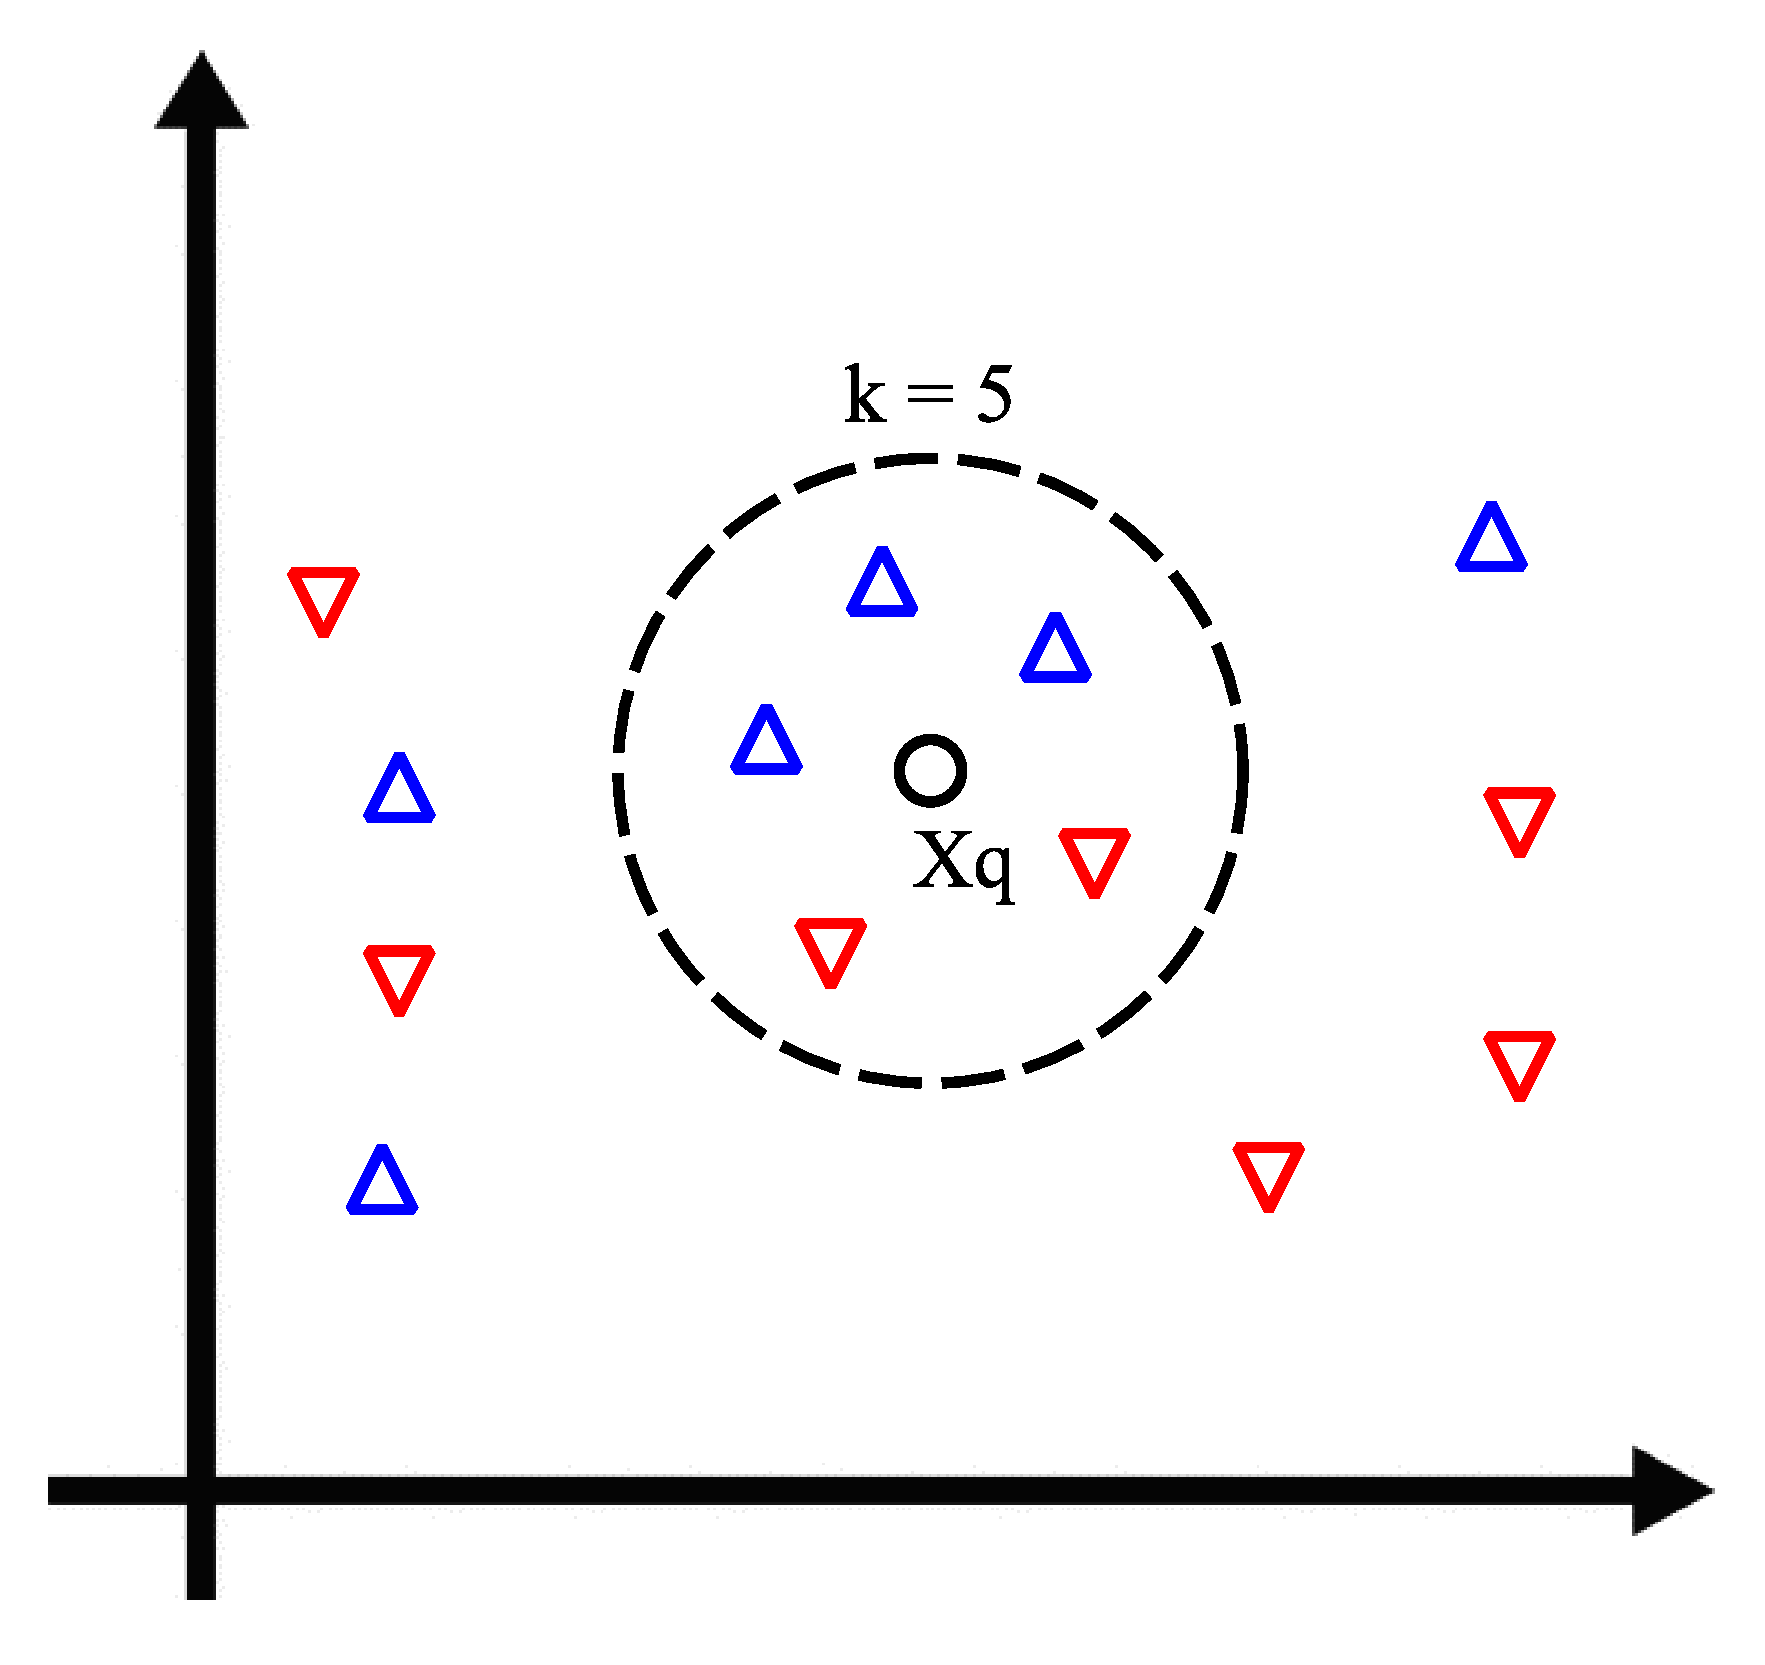
\includegraphics[width=0.6\linewidth]{knn_esquema.eps}\\
	{\small Fonte: Elaborado pelo Autor (2018).}
	\label{fig:knn_esquema}
\end{figure}

\subsection{Florestas Aleatórias}

Florestas Aleatórias (tradução literal de \textit{Randon Forest}) é uma técnica de inteligência computacional para classificação e regressão introduzido por~\citeonline{Breiman2001} que consiste no agrupamento de diversas árvores de decisão~\cite{safavian1991survey} de maneira que sua estrutura seja composta de forma aleatória (ver Figura~\ref{fig:rf_esquema}). Em árvores de decisão comuns, cada nó é dividido de modo a se obter a melhor divisão entre as variáveis do problema em questão. Por sua vez, florestas aleatórias cada nó é dividido usando o melhor entre os subconjuntos de preditores escolhidos aleatoriamente no nó em questão. O classificador requer somente a configuração de dois parâmetros de entrada para a geração do modelo de predição: o número de árvores de decisão desejadas ($n_{tree}$) e o número de variáveis de predição ($m_{try}$) usados em cada nó para o crescimento da árvore.

\begin{figure}[!htb]
	\centering
	\caption{Representação de uma Floresta Aleatória com $n$ Árvores de Decisão.}
	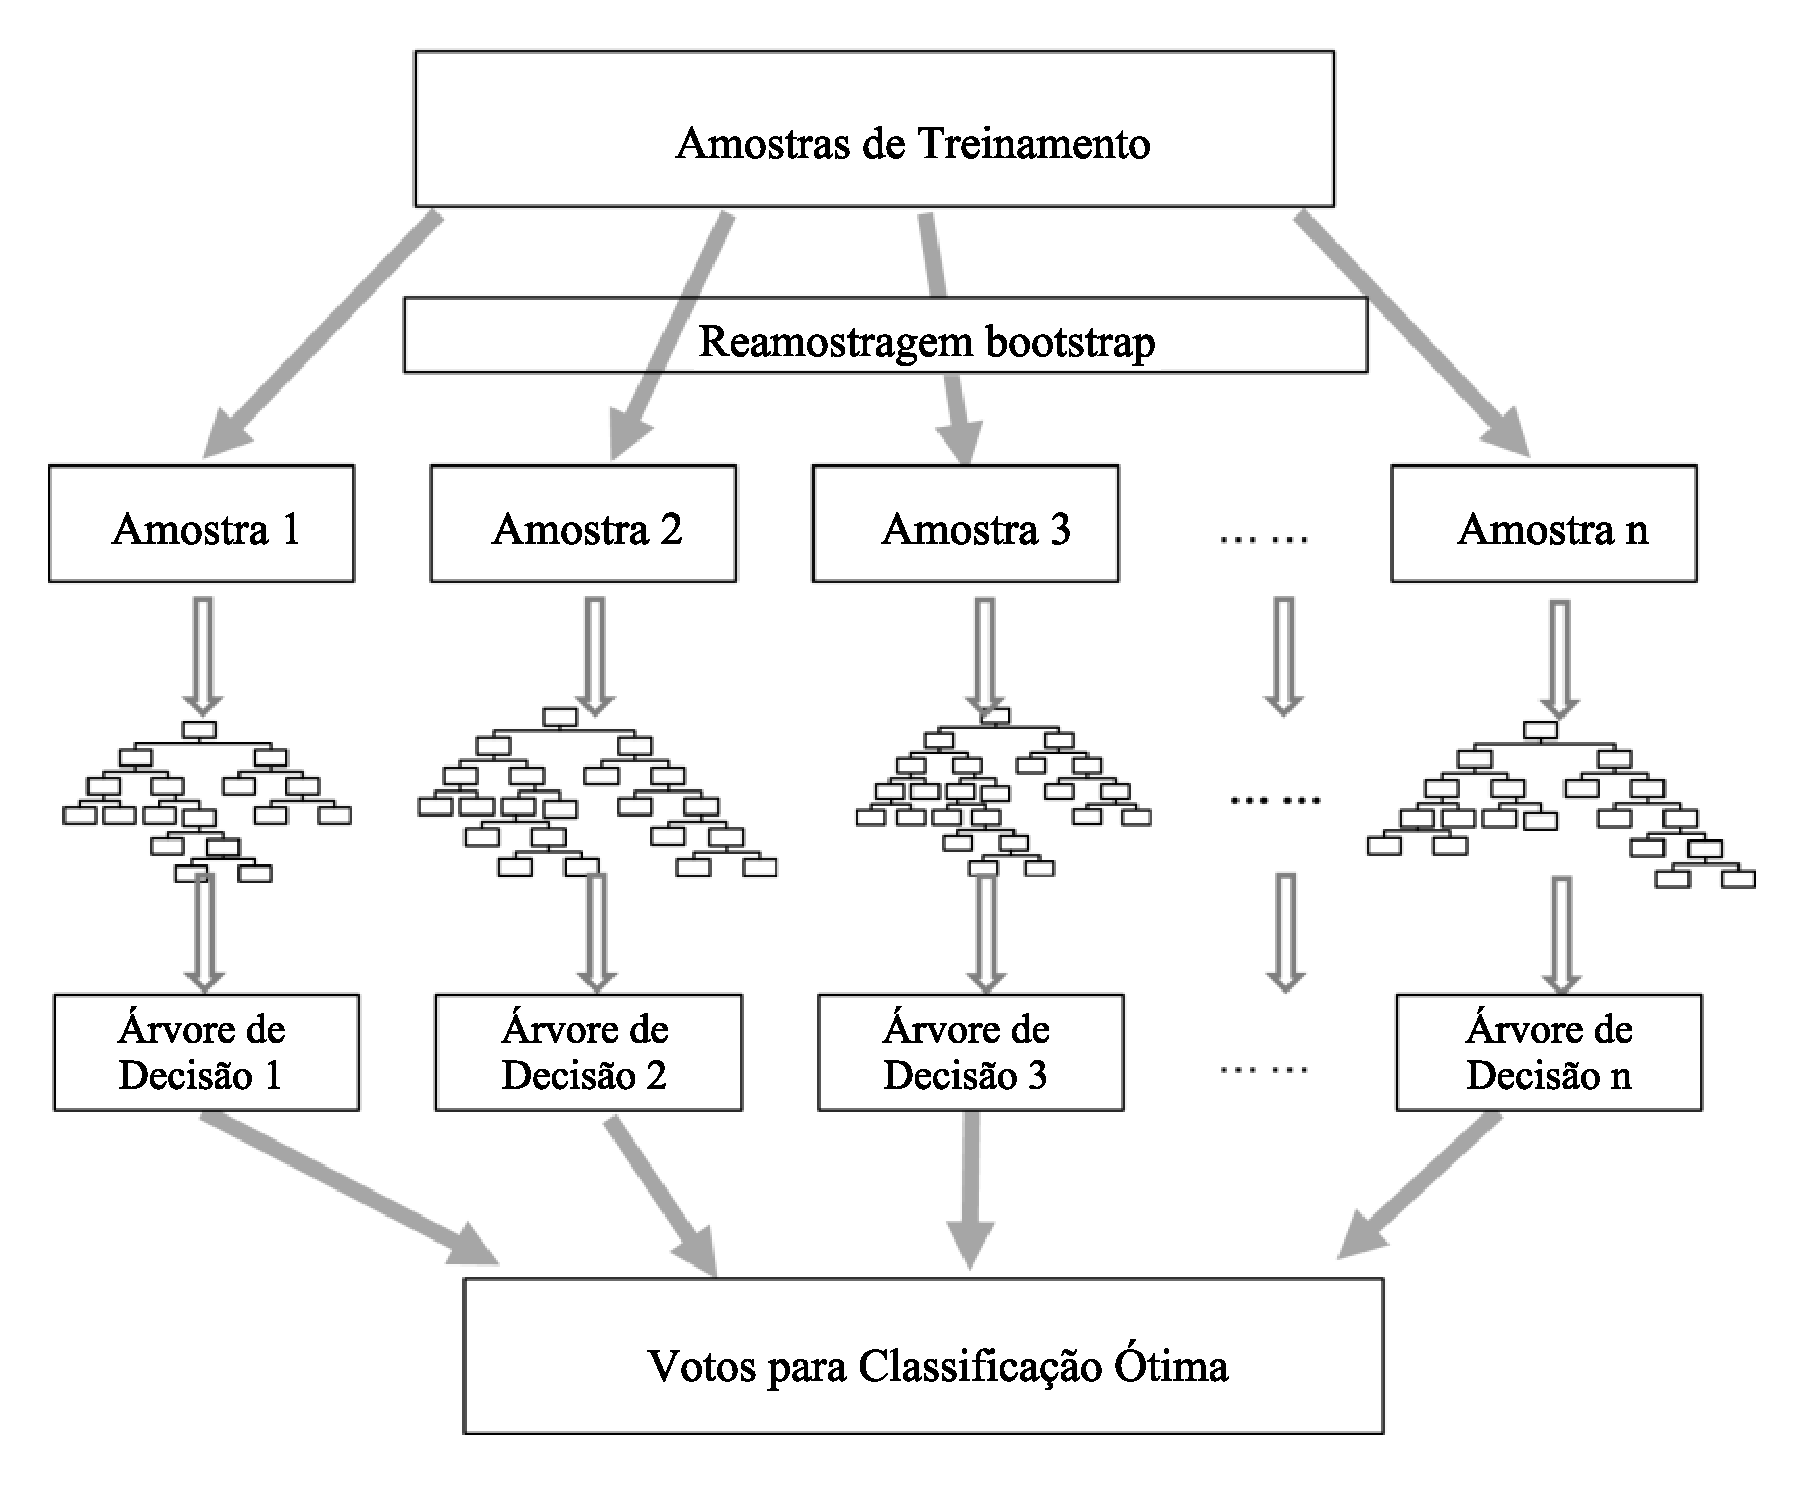
\includegraphics[width=0.8\linewidth]{RF_esquema.eps}\\
	{\small Fonte: Adaptado de \citeonline{zang2017}.}
	\label{fig:rf_esquema}
\end{figure}

Esta estratégia produz resultados satisfatórios se comparados a outros classificadores, incluindo análise discriminante, máquinas de vetor de suporte e redes neurais artificiais, além de ser robusto contra o problema de \textit{overfitting} (ou sobre-ajuste: quando um modelo se ajusta satisfatoriamente ao conjunto de dados treinado, mas se mostra ineficaz para prever novos resultados) \cite{breiman1999random} e boa imunidade à ruido gaussiano~\cite{zang2017}. Porém, apesar desta imunidade com relação ao \textit{overfitting} as florestas aleatórias tendem a saturarão do erro final, isto é, o erro se estagna em um ponto mesmo com a inserção de novas árvores à floresta.
 

\subsection{Redes Neurais Artificiais}

Umas das mais difundidas técnicas de Aprendizado de Máquina, as Redes Neurais Artificiais (RNAs) são amplamente empregadas na solução de diversos problemas de regressão e classificação, atribuindo seu sucesso à sua flexibilidade de síntese de mapeamento multidimensional não-linear de varáveis dependentes e independentes, devido a sua capacidade de aproximação universal.

RNAs são formadas por conjuntos de diversos neurônios artificais, estes propostos por McCulloch e Pitts em 1943. Este modelo de neurônio consiste em receber sinais de entrada $x_n$ nos dentritos do neurônio e retorna um único sinal de saída $y$ no axônio do mesmo. Este modelo é apresentado na Figura~\ref{fig:neuronio-artificial}.

\begin{figure}[!htb]
	\centering
	\caption{Representação de um neurônio artificial não linear.}
	\includegraphics[width=0.6\linewidth]{neuronio-artificial.jpg}\\
	{\small Fonte: Adaptado de \citeonline{haykin2009neural}.}
	\label{fig:neuronio-artificial}
\end{figure}

A expressão que representa este neurônio, com função de ativação unitária, é apresentado pela Equação~\ref{eq:neuronio},

\begin{equation}
	u_k = y_k = \sum _{i=1}^{m}{w}_{i}{x}_{i}+b
	\label{eq:neuronio}
\end{equation}

\noindent onde $x_i$ são as entradas dos neurônios, $w_i$ são os pesos das entradas, $b$ é o \textit{bias} e $y$ é a saída para uma função de ativação unitária. A função de ativação é o elemento que determina  a saída do neurônio em termos do potencial de ativação, muitas das vezes limitando a saída entre $\{0, 1\}$ e $\{-1, 1\}$. Dentre as funções mais utilizadas para esta operação estão as funções sigmoidal, linear, tangente hiperbólica, logarítmica e senoidal.

As combinações destes neurônios formam uma Rede Neural Artificial. Dentre as muitas arquiteturas utilizadas, a mais comum é a rede com múltiplas camadas. \citeonline{haykin2009neural} definu estas redes como sendo um conjunto de unidades sensoriais que constituem a camada de entrada, uma ou mais camadas ocultas e uma camada de saída. Estas redes são conhecidas como Perceptron Multicamadas (\textit{Multilayer Perceptron} - MLP) \cite{rosenblatt1962principles}. Na Figura~\ref{fig:mlp}, é apresentado um modelo de uma MLP com duas camadas escondidas (\textit{hidden layers}).

\begin{figure}[!htb]
	\centering
	\caption{Representação de uma MLP com duas camadas escondidas.}
	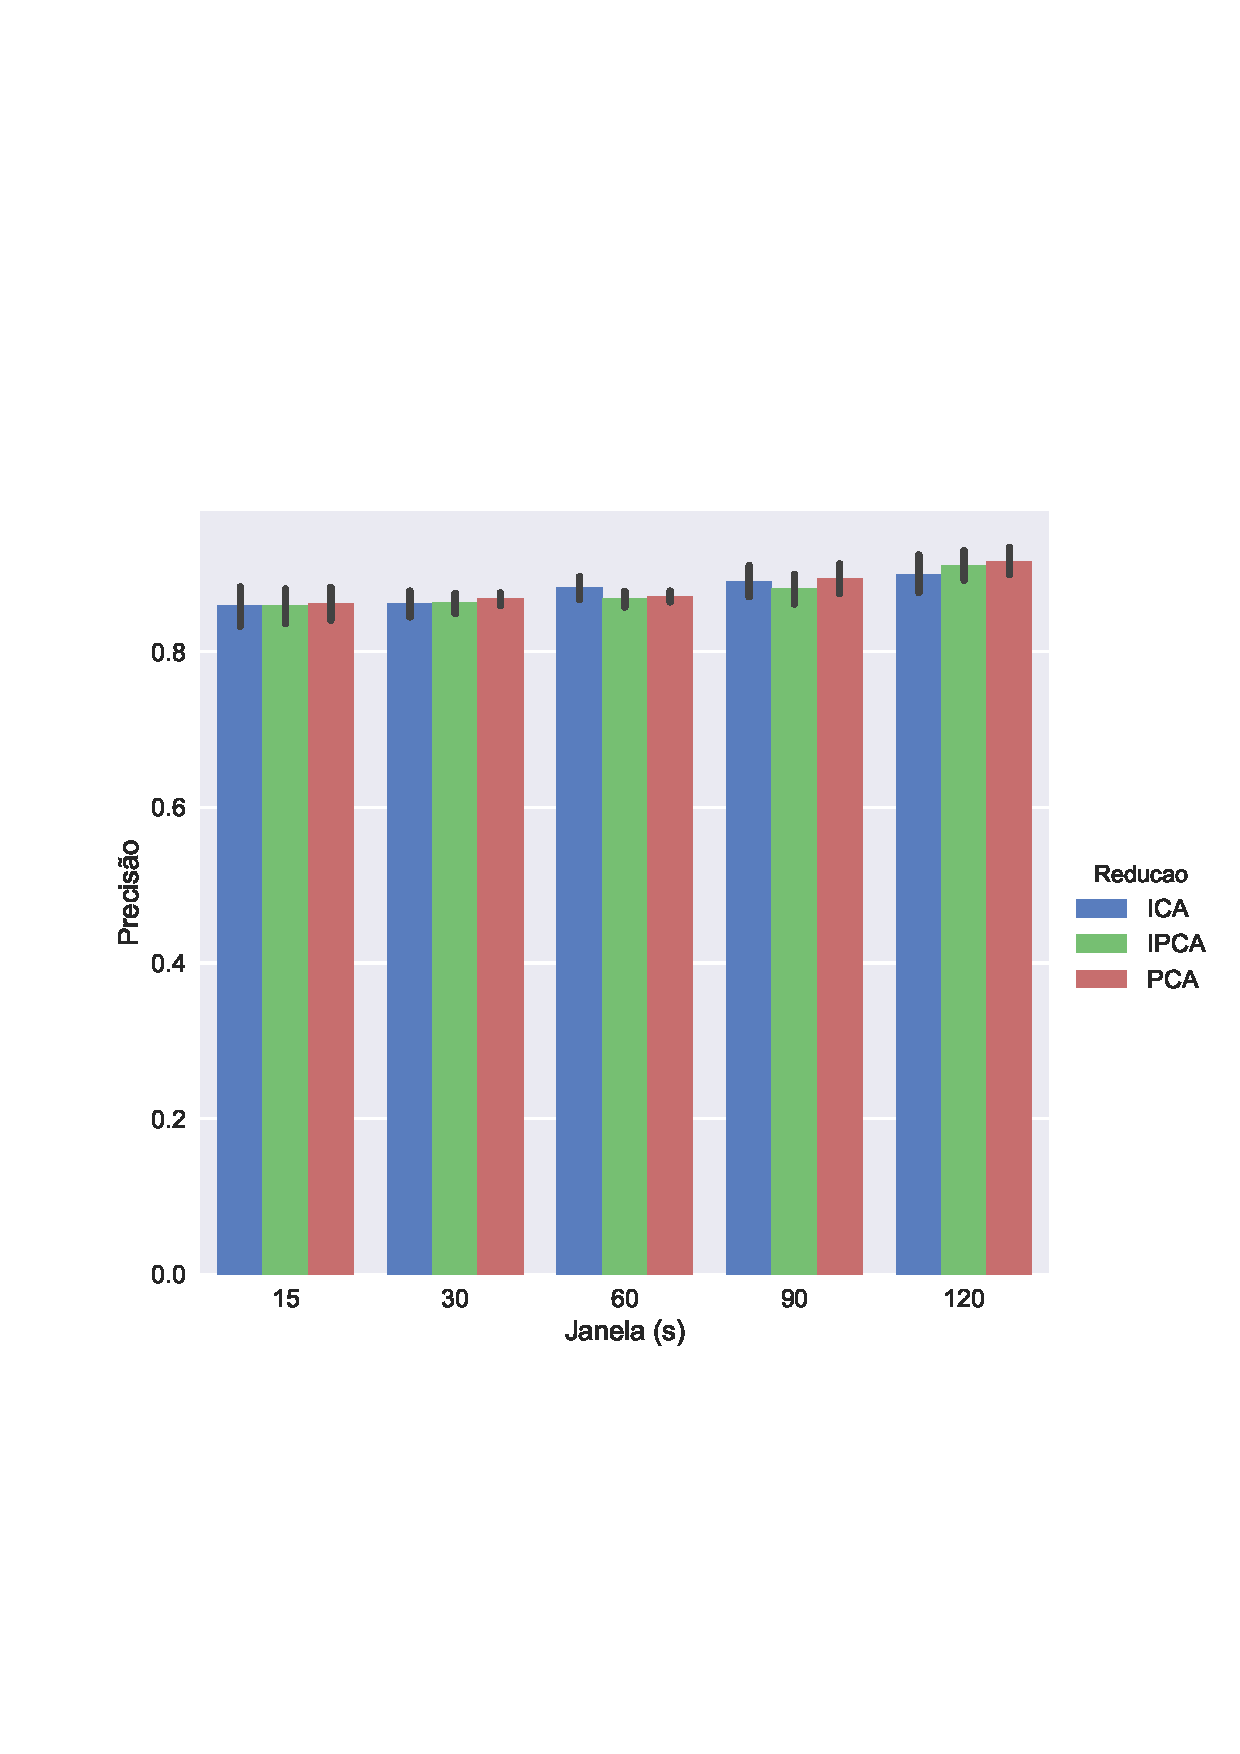
\includegraphics[width=0.8\linewidth]{MLP.png}\\
	{\small Fonte: Adaptado de \citeonline{haykin2009neural}.}
	\label{fig:mlp}
\end{figure}

Existem diveras estratégias de treinamento supervisionado para RNAs, sendo o mais difundido o algoritmo de retro-propagação de erro (\textit{error backpropagation}). Treinamento supervisionado é definido como o estímulo de uma entrada $x$ e a saída da rede $y$ é comparada com o valor desejado (valor real). A partir desta diferença os pesos são ajustados até que o resultado desejado seja obtido. Existem diversas RNAs com arquiteturas diferentes da MLP desenvolvidas, podendo-se destacar as Máquimas de Aprendizado Extremo (\textit{Extreme Learning Machines} - ELM) \cite{huang2006extreme}, Funções de Base Radial (\textit{Radial Basis Function} - RBF) \cite{powell1987algorithms} e Mapas Auto-Organizados (\textit{Self-organizing Maps} - SOM) \cite{VanHulle2012}.

\section{Algoritmos de Classificação Incrementais (\textit{Online})}

Técnicas de aprendizado não-incrementais têm algumas restrições que podem interferir no desempenho do modelo computacional, sendo estas \cite{fontenla2013online}:
\begin{enumerate}
	\item Necessidade de se ter, no momento do treinamento, todo o conjunto de dados para ajuste do modelo preditivo. A cada etapa do processo de aprendizado existe a necessidade do acesso imediato e completo do conjunto de dados.
	
	\item Não pode haver restrições de tempo, isto é, é preciso aguardar o tempo suficiente para o ajuste completo do modelo seja realizado.
	
	\item O processo subjacente aos dados de treinamento não pode sofrer mudanças. Uma vez que o modelo é ajustado, não são necessárias adaptações do mesmo desde que o processo relacionado não sofra mudanças.
\end{enumerate}

Estas restrições supracitadas se aplicam ao problema de identificação de condutores, uma vez que se trata de identificar o modo no qual o condutor opera o veículo. Este processo subjacente pode sofrer mudanças a todo o momento, dependendo de fatores temporais (horário, dia da semana) e climáticos (chuva, nevoeiro), e até mesmo alterações inerentes à estes, como uma mudança de hábitos de direção. Sendo assim, para implementações reais deste sistema, deve-se considerar outro paradigma de aprendizado de máquina para a realização da tarefa de classificação: o Aprendizado Incremental ou \textit{Online}.

Aprendizado de Máquina Incremental é um método dentro de Inteligência Computacional em que os dados tornam-se disponíveis sequencialmente e são usados para a atualização do preditor para aprimora-lo para a predição de dados futuros \cite{fontenla2013online}. A Figura~\ref{fig:apdz} apresenta graficamente a comparação do procedimento de aprendizado dos modelos de predição para algoritmos \textit{Batch} e \textit{Online}.

\begin{figure}[!htb]
	\centering
	\caption{Representação as diferenças de algoritmos de aprendizado Incremental e Não-Incremental.}
	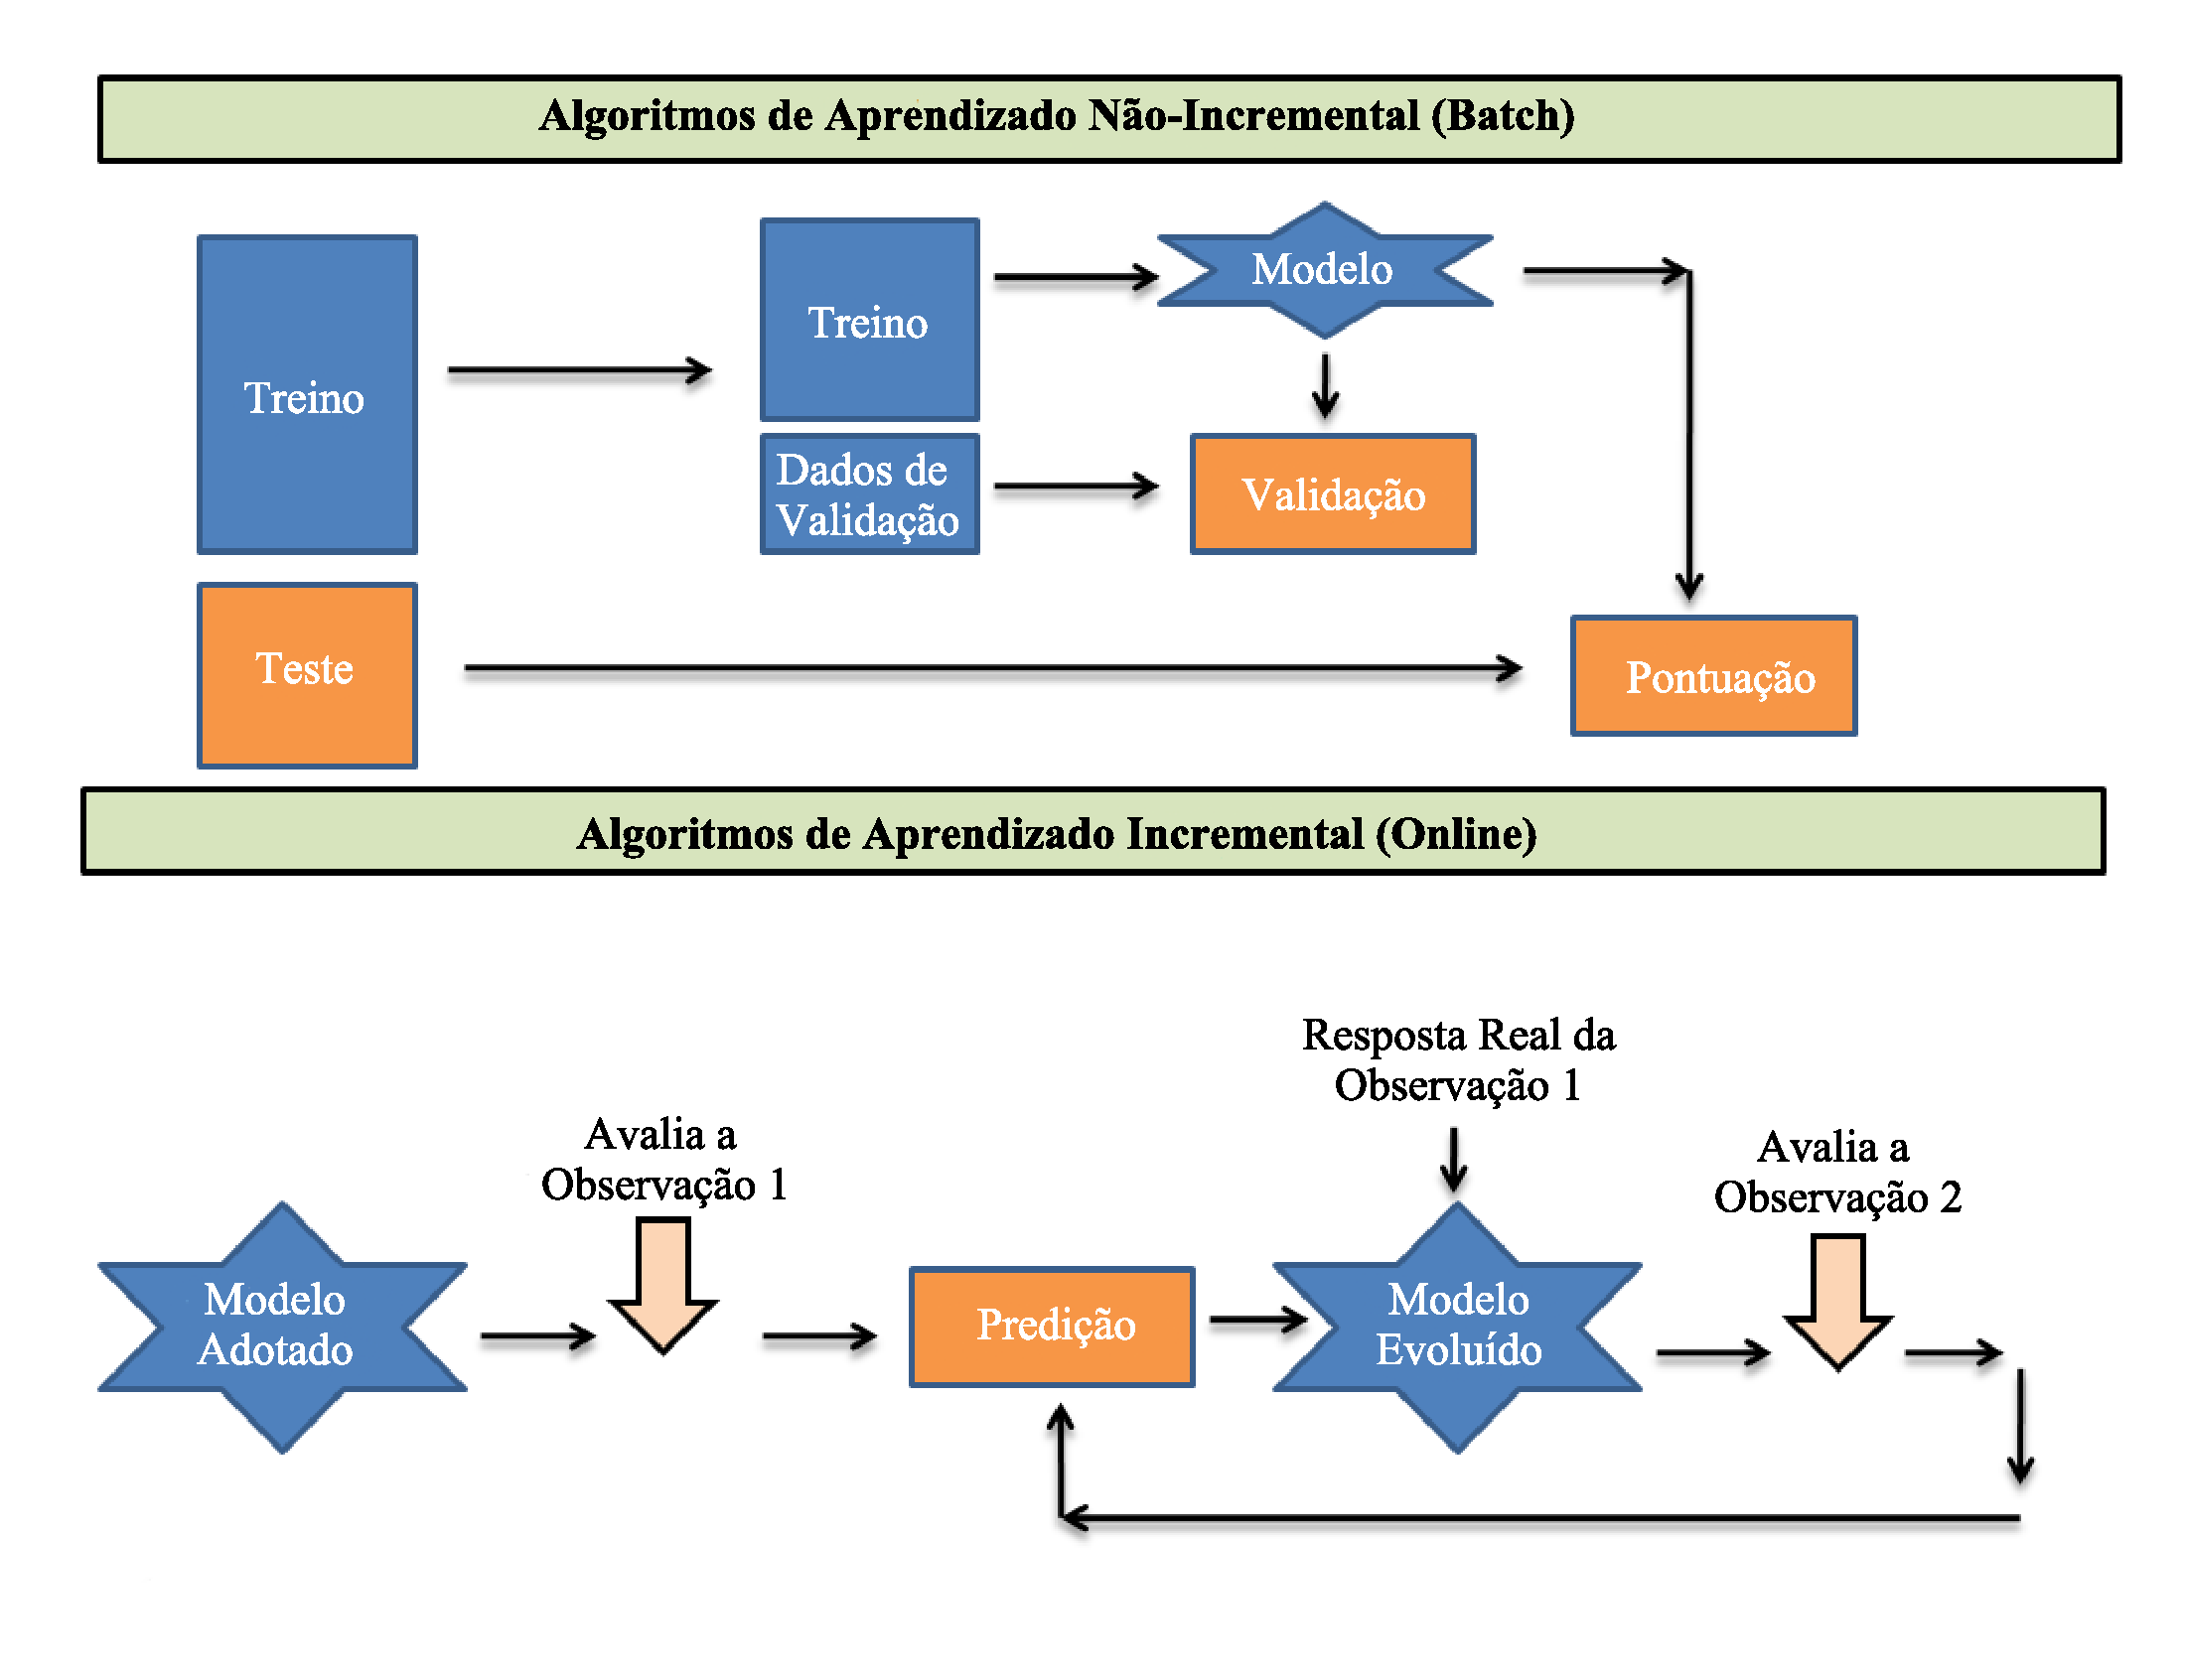
\includegraphics[width=0.9\linewidth]{aprendizado.eps}\\
	{\small Fonte: Adaptado de \citeonline{Analytics2015}.}
	\label{fig:apdz}
\end{figure}


\section{Métricas Associadas}


Para se mensurar o desempenho dos classificadores, foram considerados algumas métricas adequadas para este problema. A primeira, e mais importante, é a medida de precisão, que pode ser expressa por:

\begin{equation}
A_{cc}(R) = P(H|B) = \frac{P(HB)}{P(B)} = \frac{f_{hb}}{f_b}
\end{equation}

\noindent onde $f_{hb}$ é a quantidade de classificações corretas e $f_{b}$ é o número total de classificações. A segunda métrica utilizada é o F1-\textit{Score}, que é também uma medida de precisão, que considera também a revocação dos testes. F1-\textit{score} é obtido pela seguinte expressão:

\begin{equation}
F_1 = 2\frac{precision.recall}{precision+recall}
\end{equation}

O última medida colhida é a análise de concordância kappa (\textit{Cohen's kappa score}), que varia entre 0 e 1, os quais podem ser interpretados de acordo com a Tabela~\ref{tab:kappa}. Uma explanação mais completa destas métricas pode ser encontrado em \cite{banerjee1999beyond}.

\begin{table}[H]
	\centering
	\caption{Interpretação dos valores de Kappa}
	\label{tab:kappa}
	\begin{tabular}{ll}
		\hline
		Kappa & Interpretação \\ \hline
		\textless0 & Sem concordância \\
		0-0.19 & Concordância baixa \\
		0.20-0.39 & Concordância razoável \\
		0.40-0.59 & Concordância moderada \\
		0.60-0.79 & Concordância substancial \\
		0.80-1.00 & Concordância quase perfeita \\ \hline
	\end{tabular}
\end{table}








\chapter{CONCEITOS GERAIS}


\section{Extração de Características}

Em aprendizado de máquina, reconhecimento de padrões e processamento de imagem, extração de características começa por um conjunto inicial de dados medidos e retorna valores derivados (características) com a intenção de serem informativas e não redundantes, facilitando assim o subsequentes passo de aprendizagem e generalização e, em alguns casos, levando a uma melhor interpretação dos dados. 

\subsection{Estatísticas de Ordem Superior}

O termo Estatística de Ordem Superior (EOS) refere à funções que usam a terceira potência ou superiores de uma certa amostra, diferentemente de Estatística de Ordem Inferior, que fazem uso de termos constantes, lineares e quadráticos (potências zero, um e dois). EOS pode ser definidos em termos de momentos e cumulantes. enquanto momentos são próprios para descrever sinais determinísticos, cumulantes são adequados para a análise de sinais estocásticos (dados de direção podem ser classificados como estocásticos) \cite{guedes2016non}:. 
Considere $x$ como um processo aleatório, real e discreto com média zero. Então, a segundo, terceiro e quarto cumulante podem ser obtidos, respectivamente por 

Dado um caso unidimensional ($d = 1$), os momentos de uma variável aleatória $X$ podem ser definidos como:

\begin{equation}
    \begin{matrix}
        m_1 = \left \langle x \right \rangle\\ 
        m_2 = \left \langle x^{2} \right \rangle\\ 
        \vdots \\ 
        m_n = \left \langle x^{n} \right \rangle
    \end{matrix}
\end{equation}

Então os cumulantes podem ser escritos em forma de momentos:

\begin{equation}
\begin{matrix}
c_1 = m_1\\ 
c_2 = m_2-{m_1}^2=\sigma^2\\ 
c_3 = m_3-3{m_1}{m_2}+2{m_1}^3\\ 
c_4 = m_4 - 3{m_2}^2-4m_1m_3+12{m_1}^2m_2-6{m_1}^4
\end{matrix}
\end{equation}

Os cumulantes $c_1$, $c_2$, $c_3$ e $c_4$ são a média, a variância, a assimetria e a curtose, respectivamente. Dentre os quais somente a média não é uma EOS. Para um sinal discreto $x[n]$, os cumulantes podem ser obtidos ed forma direta por:

\begin{equation}
    C_{2,x}(\tau) = \frac{1}{N}\sum_{n=0}^{N-1}x[n]x[mod(n+\tau,N)],
    \label{eq:Dcum2}
\end{equation}

\begin{equation}
    C_{3,x}(\tau) = \frac{1}{N}\sum_{n=0}^{N-1}x[n]x^2[mod(n+\tau,N)],
    \label{eq:Dcum3}
\end{equation}

\begin{equation} \label{eq:cum4}
\begin{split}
    C_{4,x}(\tau) = \frac{1}{N}\sum_{n=0}^{N-1}x[n]x^3[mod(n+\tau,N)]-\\
    3\frac{1}{N^2}\sum_{n=0}^{N-1}x[n]x[mod(n-\tau,N)].\sum_{n=0}^{N-1}x^2[n]
\end{split}
\end{equation}

\noindent onde $x \in \Re^N$, $\tau=[0, 1,...,N-1]$ são os atrasos, e $mod$ é o operador módulo, que retorna o resto de uma operação inteira \cite{moreirahos}.

Como descrito em~\citeonline{mendel1991}, EOS pode levar a resultados mais representativos quando aplicadas como ferramenta de extração de características em processos não lineares e não gaussianos. De acordo com~\citeonline{naves2016}, a maior vantagem do uso dos cumulantes como extrator de características em problemas de classificação é sua propriedade de imunidade à ruido gaussiano.


\section{Seleção de variáveis e Redução de Dimesionalidade}

Uma ferramenta importante para melhorar a eficiência da tarefa de classificação em termos de custo computacional é a redução de dimensionalidade. Esta ferramenta pode ser definida como o processo de redução do número de variáveis de entrada pela obtenção de um conjunto de variáveis principais. Em outros termos, estas técnicas transformam um conjunto de dados de amplo espaço dimensional em um espaço de menor dimensão.

A técnica mais utilizada para redução de dimensionalidade é a Análise de Componentes Principais, descrita posteriormente neste trabalho. Outra técnica que pode ser explorada para esta tarefa é a Análise de Componentes Independentes, embora esta não seja convencionalmente usada para redução de dimensionalidade, mas para a separação de sinais sobrepostos. Contudo, existem exemplos na literatura que aplicam ICA para redução de dimensionalidade \cite{wang2006independent} \cite{cao2003comparison}.

\subsection{Análise de Componentes Principais}

PCA é um procedimento matemático que usa uma transformação ortogonal para para converter um conjunto de variáveis possivelmente correlatadas em um conjunto de variáveis não correlacionadas chamadas de componentes principais \cite{wold1987principal}. Sejam $x_t$($t=1,\ldots,l$ e $\sum_{t=1}^{l}{x_t}=0$) um conjunto de vetores de entrada de $m$ dimensões ${x_t}=({x_t}(1),{x_t}(2),\ldots,{x_t}(m))^T$, então PCA transforma linearmente $x_t$ em um novo vetor $s_t$ pela seguinte expressão:

\begin{equation}\label{eq:pca1}
	{s_t} = {U^T}{x_t},
\end{equation}
onde $U$ im uma matriz ortogonal de  $m \times m$ dimensões no qual a  $i$-ésima coluna $u_i$ é o $i$-ésimo autovetor da matriz de covariância  $C$. Portanto, PCA primeiro soluciona o problema dos autovalores:

\begin{equation}\label{eq:pca2}
	{\lambda _i}{u_i} = C{u_i}, \qquad i=1,\ldots,m,
\end{equation}
onde $\lambda _i$ é o $i$-ésimo autovalor de $C$ e ${u_i}$ é seu o autovetor relativo. Então, os componentes de ${s_t}$, baseado no obtido em ${u_i}$, são calculados como a transformação ortogonal de ${x_t}$ por:

\begin{equation}\label{eq:pca3}
	{s_t}(i) = {u_i}^T{x_t}, \qquad i=1,\ldots,m.
\end{equation}
Estes novos componente ${s_t}(i)$ são os componentes principais. Tal qual a Equação \ref{eq:pca3} demonstra, o número de componentes principais de $s_t$ pode ser reduzido pelo uso de somente alguns dos primeiros autovetores ordenados na ordem descendente dos autovalores. Assim, pode-se concluir que PCA tem a característica de reduzir a dimensão de um conjunto de dados \cite{cao2003comparison}. 

\subsection{PCA Incremental}

O PCA é uma ferramenta útil para problemas para redução de dimensionalidade, porém possui certa limitações quando utilizados em datasets maiores. Isto se dá porque o processamento do PCA é efeito em lotes, que faz com que todos os dados a serem processados devam ser armazenados na memória do dispositivo utilizado. Isto pode ser um problema para aplicações em \textit{hardware} embarcado que tem limitações quanto a capacidade de memória \cite{scikit-learn}.

Diante deste problema, a técnica de PCA Incremental (IPCA) contorna este problema, utilizando uma forma diferente de processamento  que permite cálculos parciais que praticamente obtém nos mesmo resultado do PCA, porém realizando o processamento em mini lotes \cite{Weng2003}.

A versão incremental do algoritmo funciona da seguinte maneira: assume-se que já de posse do conjunto de autovetores $U = [u_j], j = 1,\ldots, p$ do vetor de entrada $x_i, i = 1,\ldots,n$. os autovalores correspondentes são $\lambda = diag(\Lambda)$ e a média dos valores é $\overline{x}$. A construção dos incrementos requer a atualização destes autovalores e autovetores levando em conta uma nova entrada $x_{n+1}$. Primeiramente é feita atualização da média por meio da seguinte expressão\cite{Artac2002}:

\begin{equation}\label{eq:ipca1}
	\overline{x}' = \frac{1}{n+1}(n\overline{x} + x_{n+1})
\end{equation}

A atualização dos autovetores é feito pela adição do novo vetor e a aplicando uma transformação rotacional. Para tal, calcula-se o vetor ortogonal residual $h_{n+1} = (Ua_{n+1} + \overline{x})-x_{n+1}$ e em seguida sua normalização $\hat{h}_{n+1}'$. A nova matriz $U'$ é calculada por:

\begin{equation}\label{eq:ipca1}
	U' = [U \hat{h}_{n+1}] R,
\end{equation}
\noindent onde $R$ é a matriz de rotação. Este processo é repetido de acordo com o tamanho de lotes definidos (\textit{batch size}). Isto resulta em um processamento mais eficiente em termos de utilização de memória \cite{NIPS2013_5132}.

\subsection{Análise Componentes Independentes}

Análise Componentes Independentes (ICA) \cite{lee1998independent} é uma técnica que originalmente foi desenvolvida para separação cega de fontes, que recupera sinais mutualmente independentes, mas com fontes desconhecidas a partir de suas misturas lineares sem saber os coeficientes de mistura.

ICA considera que os dados são linearmente combinados por um conjunto de fontes independentes e estes sinais podem ser separados de acordo com sua independência estatística \cite{wang2006independent}. Seja $x_t$ a mistura linear e $s_t$ denota o sinal original, então o objetivo do ICA é estimar $s_t$ por:

\begin{equation}\label{eq:ica1}
	{s_t} = {U}{x_t},
\end{equation}

\noindent onde $U$ é a matriz $m \times m$ de separação de misturas. Os componentes retornados por $s_t$ são tão independentes estatisticamente quanto possível.

Existem um amplo número de algoritmos que foram desenvolvidos para executar o ICA. Neste trabalho, considerou-se o FastICA de ponto fixo, proposto por \citeonline{hyvarinen1999fast}. Este algoritmo é considerado um dos melhores e mais usados métodos já desenvolvidos. FastICA faz uso de informações mútuas como critério para estimar $s_t$, ao passo que também é uma medida natural de independência entre variáveis aleatórias. A maximização da negentropia (medida do grau de organização do sistema) corresponde à minimização das informações mútuas entre os componentes. Entretanto, esta negentropia não pode ser feita diretamente uma vez que as densidades de probabilidade dos componentes são desconhecidos. A explanação completa do funcionamento do algoritmo FastICA é encontrada em \cite{koldovsky2006efficient}.

As duas principais diferenças entre o PCA e o ICA são, primeiramente, os componentes retornados pelo ICA são estatisticamente independentes, não simplesmente descorrelacionadas tal qual ocorre nos gerados pelo PCA. A segunda distinção é que a matriz  de separação de misturas do ICA não é ortogonal tal qual a do PCA \cite{cao2003comparison}.

\subsection{Análise de Discriminante de Fisher}

Análise de Discriminante de Fisher (FDA) é uma técnica de redução de dimensionalidade, otimizado em termos da maximização da separação entre classes. Dado um conjunto de dados de $n \times m$ dimensões representado pela matriz $X$ com vetor coluna $x_i$, a matriz de dispersão total é dada por \cite{CHIANG20041389}:

\begin{equation}
    S_t=\sum_{i=1}^{n}(x_i - \mu)(x_i - \mu)^T
\end{equation}

\noindent onde $\mu$ é o vetor de médias totais dos elementos correspondentes às colunas de $X$. Considerando $X_j$ como o conjuntos de vetores $x_i$ que pertencem à uma determinada classe $j$, ma matriz de dispersão interna para a classe $j$ é

\begin{equation}
    S_t=\sum_{x_i\in X_j}^{n}(x_i - \mu_{j})(x_i - \mu_{j})^T
\end{equation}

\noindent onde $\mu_{j}$ é o vetor de médias para a classe $j$. Considerando $c$ o número de classes dos dados, então

\begin{equation}
    S_w=\sum_{i=1}^{c}S_i
\end{equation}

\noindent é a matriz de dispersão entre classes, onde $n_j$ é o número de observações na classe $j$.

O primeiro vetor FDA $w_1$ pode ser determinado como:

\begin{equation}
    \underset{w_1}{\textrm{argmax}} \frac{{w_1}^TS_bw_1}{{w_1}^TS_ww_1}
\end{equation}

O segundo vetor FDA é calculado de modo a maximizar a dispersão entre classes enquanto minimiza a dispersão entre classes entre todos os eixos perpendiculares com o primeiro vetor FDA em seguida com os vetores FDA restantes. Pode ser provado matematicamente que os vetores FDA são iguais aos autovetores $w_k$ do problema de autovalores generalizados

\begin{equation}
    S_bw_k = \lambda_jS_ww_k,
\end{equation}

\noindent onde os autovalores $\lambda_k$ indicam o grau geral de separabilidade entre as classes pela projeção de todas as classes em $w_k$. Com os vetores FDA calculados, as observações são então classificadas de forma a reduzir o espaço dos vetores FDA por meio de uma análise discriminante \cite{sugiyama2007dimensionality}.





\chapter{METODOLOGIA}
\label{cap:metodologia}

Este capítulo descreve a metodologia e as técnicas que serão empregados na pesquisa e desenvolvimento do sistema proposto, destacando as tecnologias e dispositivos necessários.

\section{Visão geral do sistema proposto}

O Sistema de Identificação de Condutores baseado em Técnicas de Inteligência Computacional terá a função de efetuar a identificação do condutor que dirige o veículo e detectar possíveis situações de roubo e furto do mesmo. Para tal, a identificação será feita por meio do reconhecimento de certos padrões de direção característicos e cada condutor. Isto é possível através da coleta de dados provenientes do barramento de comunicação do veículo, por meio da interface OBD-II e coletados pelo dispositivo de leitura ELM327, que transmite via \textit{bluetooth} para o \textit{smartphone} a ele conectado, que também fornece dados referentes à dinâmica de direção.

Um aplicativo no sistema operacional móvel Android recolherá os dados e então se formará um banco de dados referentes ao condutor. Antes de submeter os dados no algoritmo de identificação, será efetuado um processamento e fusão destes dados, a fim de remover ruídos e possíveis \textit{outliars}, além de melhorar a extração de características pelo sistema. Feito isso, o algoritmo de identificação irá cadastrar o condutor (em um primeiro momento), treinando-o com as características do mesmo, ou identificando a autenticidade do condutor em questão. O aplicativo retornará o veredicto com relação ao condutor e tomará as medidas necessárias. A Figura~\ref{fig:flux} apresenta graficamente o sistema como um todo, e os passos até a identificação.

\begin{figure}[!htb]
\centering
\caption{Visão geral do Sistema de Identificação de Condutores baseado em Técnicas de Inteligência Computacional.} %legenda
\includegraphics[scale=0.16]{FLUXOGRAMA.png}\\ 
{\small Fonte: Próprio autor.} %Fonte da imagem
\label{fig:flux} %rotulo para refencia
\end{figure}

\section{Desenvolvimento preliminar}

Para o desenvolvimento inicial do sistema proposto, será utilizado o \textit{dataset} UYANIK, cordialmente cedido pelo VPALAB da Universidade de Sabanci (Istambul, Turquia) \cite{Abut2007}. Este \textit{dataset} contém dados de um grande número de condutores colhidos a partir de dados do barramento CAN, sensores inerciais e GPS e é amplamente utilizado em diversos trabalhos que envolvem identificação de condutores \cite{Martinez2016a} \cite{jafarnejad2017} \cite{DelCampo2014}. Estes dados servirão para avaliar a aptidão das técnicas de processamento de dados e de inteligência computacional, a fim de se determinar as que melhores se encaixam na tarefa de identificação e autenticação dos condutores.

Estes resultados obtidos serão comparados com resultados quando o sistema tem como entrada dados oriundos da interface OBD-II e sensores inerciais presentes nos \textit{smarphones}. Isto se dá uma vez que o \textit{dataset} UYANIK foi colhido por meio de equipamentos mais sofisticados, com uma amostragem maior e menos ruidosos se comparado às fontes que serão utilizadas na aplicação final. O impacto desta diferença será avaliado no desempenho do sistema.

\section{Coleta de dados}

Para o desenvolvimento do sistema proposto, inicialmente será efetuada a coleta de dados que servirão como base de dados para o restante do projeto. Estes dados serão oriundos de duas fontes, a interface OBD-II (veículo) e sensores inerciais, geoposicionamento e magnéticos presentes no \textit{smartphone}.

O termo OBD-II significa \textit{On-Board Diagnostics} de segunda geração. Trata-se de um sistema que, ligado à central eletrônica do carro, permite a leitura e transmissão de diversos tipos de dados, por meio de um dispositivo eletrônico baseado no microcontrolador ELM327, que se conecta diretamente no barramento de comunicação do veículo (normanlmente CAN-bus) efetua leituras de diversos parâmetros. De acordo com \citeonline{Abuali2016}, estas informações coletadas podem ser utilizados para análise de dados, interface com usuário e coleta de dados de sensores.

Existem diversos casos na literatura que fazem uso de dados provenientes de leituras do OBD-II. Nos trabalhos de \citeonline{Martinez2015}, \citeonline{Pan2017}, \citeonline{Blaszczyk2014}, entre outros, faz-se uso de dados coletados pelo OBD-II e aplicadas técnicas de aprendizado de máquina para reconhecimento de alguns parâmetros, como agressividade, sonolência, entre outros.

Cada vez mais estudos de modelagem de comportamento do condutor têm aliado ao uso de dados provenientes do OBD-II o uso de dados sensoriais originários de \textit{smartphones}. De acordo com \citeonline{Saiprasert2017}, a capacidade de multi-sensoriamento de smartphone disponíveis no mercado propicia a coleta de uma preciosa gama de dados brutos. Dados de acelerômetros fornecem uma visão do movimento longitudinal e lateral do celular, e consequentemente do veículo, enquanto o GPS nele embarcado pode fornecer dados de localização em termos de longitude e latitude.

Na literatura, \textit{smartphones} têm sido empregados como ferramenta de coleta e processamento de dados em vasta gama de aplicações em sistemas veiculares. \citeonline{Hong2014} desenvolveram uma plataforma de modelagem de estilos de direção baseando-se somente em dados de sensores de \textit{smartphones}. Neste caso, os autores justificam que sistemas sensoriais para tal modelagem são caros, enquanto a penetração de mercado de \textit{smartphones} está praticamente consolidada, tendo assim aplicações desta natureza acessibilidade a praticamente todos os condutores.

Ciente do potencial de aplicação destas duas fontes de dados para aplicação em modelagem e identificação de comportamento de condutores, pretende-se que o sistema faça a leitura do barramento CAN do veículo, baseado do aplicativo desenvolvido por \citeonline{Neto2016}. Para tal, será avaliado quais variáveis serão monitoras de acordo com a aptidão de cada uma delas em detectar padrões característicos do condutor. Como apresentado por \citeonline{jafarnejad2017}, alguns sinais têm representatividade na identificação de condutores, a saber:

\begin{itemize}
    \item Porcentagem do Pedal de Acelerador.
    
    \item Ângulo do Volante em graus.
    
    \item Velocidade do Veículo.
    
    \item Rotação do Motor (RPM).
    
    \item Taxa de Guinada (Yaw Rate).
    
\end{itemize}

Para veículos brasileiros, alguns destes sinais, como o ângulo do volante, podem não estar disponíveis no mesmo. Para tal, será investigado o impacto da inexistência destes no processo e outras variáveis serão avaliadas como possíveis substitutas, de modo que a taxa de acertos do condutor seja maximizada. Não existe, porém, na literatura um consenso de quais variáveis têm maior capacidade de definir padrões que podem ser importantes na identificação do condutor.

\section{Processamento de sinais}

Para a aplicação de dados em qualquer técnica de aprendizado de máquina, é imprescindível que os dados sejam submetidos à um tratamento prévio, de tal modo à remover quaisquer ruídos, erros de medição e outras irregularidades nas informações.

Alguns trabalhados adotaram somente um processamento estatístico básico, como o cálculo de média acumulada, desvio padrão e amplitude dos dados, como visto em \citeonline{Carmona2015}. Por outro lado, o trabalho desenvolvido por \citeonline{Kumtepe2016} representa os sinais em forma de funções de densidade de probabilidade e então modelaram-nos por meio de Modelo de Misturas Gaussianas (GMM). Formam-se histogramas dos dados que ainda são filtrados por meio do método das médias móveis. Segundo o autor, este método proporciona uma representação efetiva de dados de direção.

Uma técnica de processamento de dados explorada por \citeonline{DelCampo2014}, especialmente para a aplicação de identificação de condutores, é a análise cepstral, aplicada como filtro e extrator de características. A técnica também é explora para processamento de sinais para identificação de condutores por \citeonline{jafarnejad2017}, em paralelo com extração estatística de características (média, mediana, curtoses, assimetria). Ambos trabalhos ressaltam que a análise cepstral é uma técnica com potencial para aplicação em identificação de condutores, por ser leve computacionalmente e adequada para futuras implementações em sistemas embarcados. Para tanto, pretende-se avaliar técnicas de pré-processamento de dados de forma a maximizar o desempenho do sistema \cite{Ahmadi-Pour2017}.



\section{Algoritmo de Identificação de Condutores}

Após a coleta dos dados referentes à dinâmica de direção e o processamento destes com o propósito de maximizar a extração de características, chega-se à fase de identificação do condutor por meio destes dados. Isto se dará por meio do uso de técnicas de aprendizado de máquina, em forma de classificador. Este processo será dividido em duas fases: primeiramente deve-se cadastrar o condutor autorizado à utilizar o veículo, por meio do treinamento do algoritmo. Na segunda fase, com o algoritmo já treinado para um ou mais condutores autorizados, deve-se avaliar e identificar o condutor que opera o veículo no momento.

O desenvolvimento desta parte do sistema passará inicialmente pela avaliação da técnica de aprendizado de máquina mais adequada para realizar a tarefa de identificação. Para tanto, alguns requisitos serão observados:

\begin{itemize}

    \item \textbf{Taxa de acertos:} este parâmetro consiste em avaliar qual técnica tem melhor aptidão em identificar a autenticidade do condutor, sem que o mesmo seja avaliado como sendo autorizado quando não o é e vice-versa. Este é um ponto crítico o sistema, pois em aplicações reais é imprescindível que o algoritmo não cometa equívocos quanto à decisão.
    
    \item \textbf{Custo computacional:} tendo em vista que o \textit{hardware} a ser utilizado é limitado (\textit{smartphone}, sistemas embarcados, FPGA, entre outros), o custo computacional da técnica deve ser cuidadosamente avaliado. O tempo de treinamento do algoritmo (cadastro) é um dos principais pontos a serem avaliados neste parâmetro, pois o mesmo deve ser rápido, mas ao mesmo tempo eficiente, com o propósito de não comprometer o desempenho do sistema.
    
    \item \textbf{Tempo de processamento:} tendo em vista que o sistema deverá verificar a autenticidade do condutor, o tempo em que o algoritmo leva para efetuar tal identificação é um ponto crucial, pois quanto mais rápido é identificado um intruso, maiores as chances de se impedir a ação criminosa.
    
\end{itemize}

No que diz respeito à \textit{driver behavior proffiling}, não existe uma unanimidade entre os autores em relação à qual técnica de aprendizado de máquina é a mais apropriada. Conforme apresentado por \citeonline{Meiring2015}, cada aplicação que envolva algum tipo de detecção de padrões (distração, sonolência, embriagues, agressividade) possui uma ou mais técnicas que tiveram resultados satisfatórios. Como existem poucos trabalhos na área de identificação de condutores, ainda se tem em aberto a possibilidade de testes em diversas técnicas de aprendizado de máquina, respeitando as premissas supracitadas.

Serão selecionados diversos algoritmos de classificação, dos quais serão avaliados o desempenho, de acordo com os requisitos definidos. Das técnicas que serão testadas, selecionou-se algumas que obtiveram desempenho satisfatório em outros trabalhos relacionados à identificação de condutores, dentre os quais pode-se citar:

\begin{itemize}
    \item \textbf{AdaBoost}, utilizado por \citeonline{jafarnejad2017}.
    
    \item \textbf{Gradient Boosting}, utilizado por \citeonline{jafarnejad2017}.
    
    \item \textbf{Extra Trees}, utilizado por \citeonline{jafarnejad2017}.
    
    \item \textbf{\textit{Extreme Learning Machines}}, utilizado por \citeonline{Martinez2016a}.
    
    
    \item \textbf{Máquinas de Vetor de Suporte}, utilizado por \citeonline{Chen2015} e \citeonline{jafarnejad2017}.
    
    \item \textbf{Redes Neurais Artificiais}, utilizado por \citeonline{DelCampo2014}.
    
    \item \textbf{Florestas Aleatórias}, utilizado por \citeonline{Wang2017a} e \citeonline{jafarnejad2017}.

\end{itemize}

É importante salientar que outros algoritmos ainda não utilizados em outros projetos poderão ser testados, uma vez identificada sua capacidade de desempenhar a tarefa de identificação e autenticação de condutores.

\section{Desenvolvimento de aplicação móvel Android}

Todos os elementos citados anteriormente irão compor um aplicativo para sistema operacional Android, que irá desempenhar a tarefa de identificação de condutores. Para isto, o desenvolvimento do mesmo irá se basear no trabalho desenvolvido por \citeonline{Neto2016}, que consiste basicamente num aplicativo que efetua leituras do dispositivo OBD-II, por meio da interface \textit{Bluetooth}, e também recolhe informações de sensores presentes no \textit{smartphone}, tais como acelerômetro, giroscópio, bússula (sensor de orientação) e GPS.

Diversos trabalhos exploram aplicações baseadas em Android, para a realização da tarefa de modelagem do perfil de condutores. Isto se deve muito à capacidade computacional que os \textit{smartphones} possuem atualmente, aliado aptidão que os sensores presentes nos mesmos têm de realizar leitura da dinâmica de direção como um todo.

Como exemplo, o aplicativo \textit{DrivingStyles} desenvolvido por \citeonline{Meseguer2017}, que por meio destas leituras, utiliza uma rede neural artificial treinada que identifica o estilo de direção do condutor entre calmo, normal e agressivo. De forma semelhante, \citeonline{Saiprasert2017} desenvolveram um aplicativo que monitora toda a dinâmica de direção e indica possíveis comportamentos que possam ser perigosos aos usuários do veículo.

Sendo assim, o uso de aplicativos móveis é uma ferramenta poderosa para implementação de sistemas que abranjam identificação de comportamento de condutores por meio de sensores que monitorem a dinâmica de direção como um todo. Portanto, para o presente trabalho, o desenvolvimento de um aplicativo que embarque todos os elementos que serão desenvolvidos é uma forma interessante de validar o sistema de uma forma simples, eficiente e acessível a um custo relativamente baixo.

\chapter{RESULTADOS PRELIMINARES E ESPERADOS}
\label{cap:resultados}

\section{Resultados Preliminares}


Um dos objetivos do presente trabalho é testar a aptidão de diferentes técnicas de processamento e classificação de dados para tarefa de classificação de condutores. Os gráficos da Figura mostram o desempenho em termos da acurácia dos testes juntamente com a dispersão dos resultados dos classificadores, divididos em cada umas das técnicas de redução de dimensionalidade.

Em todos os cenários, o classificador KNN obteve desempenho superior em comparação aos outros classificadores, enquanto o MLP teve um desempenho consideravelmente inferior, além de apresentar valores de desvio padrão superiores, se mostrando uma técnica pouco indicada para a tarefa de identificação de condutores.

Considerando a janela temporal ideal para a identificação de condutores, conclui-se que a janela de 90 segundos maximiza o desempenho do classificador KNN, porém nos casos das técnicas MLP e RF, quanto maior a janela temporal, melhor a taxa de acertos dos mesmos. A janela temporal de 30 segundos apresentou desempenho inferior no KNN e RF, enquanto que no caso do MLP, os valores se estabilizaram a partir da janela de 30 segundo, com acréscimo razoável na janela de 120 segundo. 

Pode-se observar que a janela de 90 segundos tem o melhor desempenho no que diz respeito aos certos quanto à autenticidade do condutor. É valido ressaltar que, em aplicações reais futuras, deve-se determinar uma valor de janela ótimo que alie a rapidez e precisão na identificação do condutor, visto que uma janela de 90 segundo pode ser muito quanto se trata de uma ação criminosa, porém um falso negativo é uma situação que deve ser evitada para a confiabilidade do sistema.

Com relação à eficiência dos métodos de redução de dimensionalidade, nenhumas das técnicas se mostrou superior em questão de desempenho em relação às outras, no qual o objetivo de diminuir o espaço amostral de entrada do classificador foi alcançado sem que se houvesse comprometimento na classificação.

No caso do melhor classificador, o KNN, as três técnicas obtiveram uma quantidade de acertos semelhantes nas mesmas condições de janela temporal. Porém, nos classificadores RF e MLP não houve uma técnica que teve seu desempenho superior em todas as circunstâncias. Os gráficos apresentados na Figura ilustram o desempenho comparado de cada uma das técnicas de redução de dimensionalidade em cada um dos classificadores abordados.

Como o classificador KNN teve um desempenho consideravelmente superior aos demais, optou-se por efetuar uma análise de desempenho mais aprofundada do mesmo, considerando, além da precisão, as métricas de análise de concordância \textit{Cohen's kappa Score} e \textit{F1-Score}. Pode-se observar que em todos os casos, a janela de 90 segundos resulta em um resultado melhor chegando à 99.5\% de acertos com redução PCA e ICA e 99.4\% na redução IPCA.

\begin{table}[htb]
\centering
\caption{Desempenho do Classificador KNN e Redução de Dimensionalidade PCA em diferentes métricas}
\label{tab:desPCA}
\resizebox{0.47\textwidth}{!}{
\begin{tabular}{cccc}
\hline
\multicolumn{4}{c}{PCA} \\ \hline
\multirow{2}{*}{Janela (s)} & \multicolumn{3}{c}{KNN} \\ \cline{2-4} 
 & Acurácia & F1-Score & Cohen Kappa \\ \hline
15 & 0.956 $\pm$ 0 & 0.927 $\pm$ 0 & 0.896 $\pm$ 0 \\
30 & 0.919 $\pm$ 0 & 0.838 $\pm$ 0 & 0.785 $\pm$ 0 \\
60 & 0.971 $\pm$ 0 & 0.951 $\pm$ 0 & 0.930 $\pm$ 0 \\
90 & 0.995 $\pm$ 0 & 0.992 $\pm$ 0 & 0.988 $\pm$ 0 \\
120 & 0.989 $\pm$ 0 & 0.981 $\pm$ 0 & 0.974 $\pm$ 0 \\ \hline
\end{tabular}}
\end{table}

\begin{table}[htb]
\centering
\caption{Desempenho do Classificador KNN e Redução de Dimensionalidade IPCA em diferentes métricas}
\label{tab:desIPCA}
\resizebox{0.47\textwidth}{!}{
\begin{tabular}{cccc}
\hline
\multicolumn{4}{c}{IPCA} \\ \hline
\multicolumn{1}{l}{\multirow{2}{*}{Janela (s)}} & \multicolumn{3}{c}{KNN} \\ \cline{2-4} 
\multicolumn{1}{l}{} & \multicolumn{1}{l}{Acurácia} & \multicolumn{1}{l}{F1-Score} & \multicolumn{1}{l}{Cohen Kappa} \\ \hline
15 & 0.956 $\pm$ 0 & 0.927 $\pm$ 0 & 0.896 $\pm$ 0 \\
30 & 0.922 $\pm$ 0 & 0.842 $\pm$ 0 & 0.7905 $\pm$ 0 \\
60 & 0.972 $\pm$ 0 & 0.952 $\pm$ 0 & 0.932 $\pm$ 0 \\
90 & 0.994 $\pm$ 0 & 0.990 $\pm$ 0 & 0.986 $\pm$ 0 \\
120 & 0.989 $\pm$ 0 & 0.981 $\pm$ 0 & 0.974 $\pm$ 0 \\ \hline
\end{tabular}}
\end{table}

\begin{table}[htb]
\centering
\caption{Desempenho do Classificador KNN e Redução de Dimensionalidade ICA em diferentes métricas}
\label{tab:desICA}
\resizebox{0.47\textwidth}{!}{
\begin{tabular}{cccc}
\hline
\multicolumn{4}{c}{ICA} \\ \hline
\multirow{2}{*}{Janela (s)} & \multicolumn{3}{c}{KNN} \\ \cline{2-4} 
 & Acurácia & F1-Score & Cohen Kappa \\ \hline
15 & 0.957 $\pm$ 0 & 0.927 $\pm$ 0 & 0.896 $\pm$ 0 \\
30 & 0.917 $\pm$ 0 & 0.834 $\pm$ 0 & 0.778 $\pm$ 0 \\
60 & 0.976 $\pm$ 0 & 0.960 $\pm$ 0 & 0.943 $\pm$ 0 \\
90 & 0.995 $\pm$ 0 & 0.991 $\pm$ 0 & 0.988 $\pm$ 0 \\
120 & 0.988$ \pm$ 0 & 0.980 $\pm$ 0 & 0.971 $\pm$ 0 \\ \hline
\end{tabular}}
\end{table}


\section{Resultados esperados}

Espera-se com os resultados desta pesquisa, desenvolver um sistema, que, através de técnicas de inteligência computacional, possa identificar, autenticar e discernir condutores por meio de sinais presentes no barramento CAN e \textit{smartphones}. Para tanto, como produto final desta pesquisa, espera-se o desenvolvimento de um aplicativo móvel que desempenhe as tarefas mencionadas, com uma alta taxa de acertos na autenticação dos condutores. Estes resultados poderão contribuir para a implementação futura em larga escala do sistema em \textit{hardware} embarcado no veículo, podendo contribuir para a mitigação de roubos e furtos de veículos, além de outras aplicações. Também espera-se a publicação de um ou mais artigos ou resumos expandidos em periódicos ou congressos da área de Engenharias IV.

\chapter{EQUIPE}
\label{cap:equipe}

A equipe de pesquisadores que irá trabalhar na pesquisa e desenvolvimento no presente projeto está descrito na Tabela~\ref{tab:equipe}.

\begin{table}[!htb]
	\centering
	\caption{Cronograma das atividades que serão realizadas.}
	\label{tab:equipe}
	\begin{tabular}{ccc}
\hline
Nome & Título & Instituição \\ \hline
Wilian Soares Lacerda (Orientador) & Doutor & UFLA \\
Andrey Gustavo de Souza & Mestrando & UFLA \\ \hline
\end{tabular}\\
\centering {\small Fonte: Próprio autor.} %Fonte do quadro
\end{table}

Poderá-se avaliar a necessidade da inclusão de outros membros à equipe de pesquisa, dentre coorientadores e alunos de iniciação científica, de acordo com as demandas identificadas no andamento do projeto.

\chapter{ORÇAMENTO}
\label{cap:orcamento}

Para o desenvolvimento desta pesquisa, serão usado \textit{softwares} de uso gratuito (Python, Android Studio) ou que estão disponíveis para uso através do Departamento de Engenharia (DEG) da Universidade Federal de Lavras (UFLA) (Matlab).  Os equipamentos que serão necessários para a implementação já foram adquiridos ou estão disponíveis pelos Laboratórios da UFLA, conforme descrito na Tabela~\ref{tab:orca}. Os veículos que serão utilizados para os testes e validação do sistema serão disponibilizados por meio de voluntários que se dispuserem a testar o sistema.

\begin{table}[!htb]
	\centering
	\caption{Equipamentos necessários para desenvolvimento do projeto.}
	\label{tab:orca}
\begin{tabular}{cc}
\hline
\multicolumn{1}{c}{Equipamento} & Fonte/Proprietário \\ \hline
Microcomputador & Pesquisador/LABSINE (UFLA) \\
Aparelho Smartphone & Pesquisador \\
Leitor OBD-II & Pesquisador/LMT (UFLA) \\ \hline
\end{tabular}\\
\centering {\small Fonte: Próprio autor.} %Fonte do quadro
\end{table}

\chapter{CRONOGRAMA}
\label{cap:crono}

Com início no primeiro período de 2017 (maio), o programa de Mestrado se iniciou com a escolha do tema da dissertação, sendo definido o título do presente projeto de pesquisa. Juntamente com o orientador, foram definidas as disciplinas que seriam cursadas. No primeiro período de 2017 foram cursadas as disciplinas: PCH501 Inglês Instrumental, PSI505 Tópicos Especiais em Engenharia de Sistemas e Automação (Redes Neurais Artificiais), PSI515 Pesquisa Bibliográfica e Comunicação Científica, PSI528 Processamento de Sinais e PSI531 Sistemas Fuzzy. No segundo período de 2017 foram cursadas as seguintes disciplinas: PSI504 Seminário I, PSI511 Estágio Docência I MS, PSI514 Projeto Orientado, PSI516 Computação Evolucionária, PSI519 Análise de Componentes Independentes e PSI535 Eletrônica de Potência Aplicada a Sistemas Elétricos. Estas disciplinas integralizam a carga horária mínima obrigatória de 24 créditos. 

Dando continuidade ao trabalho que resultará no dissertação de mestrado, é determinado o cronograma apresentado na Tabela~\ref{tab:crono}, com as seguintes atividades:

\begin{enumerate}
	\item Início do mestrado.
	
	\item Cumprimento da carga horária mínima exigida em disciplinas.
	
    \item Revisão da literatura, construção de acervo bibliográfico e análise do estado da arte do sistema proposto.
    
    \item Escrita do Projeto de Qualificação.
    
    \item Avaliação e implementação de testes preliminares de métodos de processamento de dados e algoritmo de identificação de condutores.
    
    \item Avaliação da viabilidade do sistema de identificação de condutores por meio dos resultados preliminares.
    
    \item Exame de Qualificação.
    
    \item Avaliação de técnicas de aprendizado \textit{online} a serem implementadas.
    
    \item Implementação e testes com as técnicas escolhidas e definição da técnica a ser utilizada no sistema.
    
    \item Teste e validação do sistema proposto, através de experimentos e avaliação dos resultados.
    
    \item Escrita da dissertação.
    
    \item Defesa da dissertação.
    
\end{enumerate}

\begin{table}[h]
	\centering
	\caption{Cronograma das atividades que serão realizadas.}
	\label{tab:crono}
\resizebox{\textwidth}{!}{\begin{tabular}{|c|c|c|c|c|c|c|c|c|c|c|c|c|c|c|c|c|c|c|c|c|c|c|}
		\hline
		\multirow{2}{*}{Atividade} & \multicolumn{8}{c|}{2017} & \multicolumn{12}{c|}{2018} & \multicolumn{2}{c|}{2019} \\ \cline{2-23} 
		& Maio & Jun. & Jul. & Ago. & Set. & Out. & Nov. & Dez. & Jan. & Fev. & Mar. & Abr. & Maio & Jun. & Jul. & Ago. & Set. & Out. & Nov. & Dez. & Jan. & Fev. \\ \hline
		1 & X &  &  &  &  &  &  &  &  &  &  &  &  &  &  &  &  &  &  &  &  &  \\ \hline
		2 & X & X & X & X & X & X & X & X & X & X &  &  &  &  &  &  &  &  &  &  &  &  \\ \hline
		3 &  &  &  &  & X & X & X & X & X & X & X &  &  &  &  &  &  &  &  &  &  &  \\ \hline
		4 &  &  &  &  &  &  & X & X & X & X & X & X &  &  &  &  &  &  &  &  &  &  \\ \hline
		5 &  &  &  &  &  & X & X & X & X & X & X &  &  &  &  &  &  &  &  &  &  &  \\ \hline
		6 &  &  &  &  &  &  &  &  &  &  &  & X &  &  &  &  &  &  &  &  &  &  \\ \hline
		7 &  &  &  &  &  &  &  &  &  &  &  &  & X &  &  &  &  &  &  &  &  &  \\ \hline
		8 &  &  &  &  &  &  &  &  &  &  &  &  &  & X & X & X &  &  &  &  &  &  \\ \hline
		9 &  &  &  &  &  &  &  &  &  &  &  &  &  &  &  & X & X & X &  &  &  &  \\ \hline
		10 &  &  &  &  &  &  &  &  &  &  &  &  &  &  &  &  &  & X & X & X &  &  \\ \hline
		11 &  &  &  &  &  &  &  &  &  &  &  &  &  &  & X & X & X & X & X & X & X &  \\ \hline
		12 &  &  &  &  &  &  &  &  &  &  &  &  &  &  &  &  &  &  &  &  &  & X \\ \hline
\end{tabular}}
\centering {\small Fonte: Próprio autor.} %Fonte do quadro
\end{table}
%==============================================================================
% Incluindo bibliografia
%\bibliographystyle{plain}             % estilo para labels em numeros
%\bibliographystyle{alpha}             % estilo para labels em iniciais
\bibliographystyle{abntex2-alf}           % estilo para referências usando ABNT, 
                                       % precisa instalar o abntex para usar!!!

%inclui Referências Bibliográficas
%inclui Referências Bibliográficas
\referencias
\bibliography{refbib}			% arquivo exemplo refbib.bib



%==============================================================================
% Incluindo anexos num1erados com letras maiusculas.
%\apendices





%==============================================================================
% Fim do texto
\end{document}
